% Options for packages loaded elsewhere
\PassOptionsToPackage{unicode}{hyperref}
\PassOptionsToPackage{hyphens}{url}
%
\documentclass[
]{article}
\usepackage{lmodern}
\usepackage{amssymb,amsmath}
\usepackage{ifxetex,ifluatex}
\ifnum 0\ifxetex 1\fi\ifluatex 1\fi=0 % if pdftex
  \usepackage[T1]{fontenc}
  \usepackage[utf8]{inputenc}
  \usepackage{textcomp} % provide euro and other symbols
\else % if luatex or xetex
  \usepackage{unicode-math}
  \defaultfontfeatures{Scale=MatchLowercase}
  \defaultfontfeatures[\rmfamily]{Ligatures=TeX,Scale=1}
\fi
% Use upquote if available, for straight quotes in verbatim environments
\IfFileExists{upquote.sty}{\usepackage{upquote}}{}
\IfFileExists{microtype.sty}{% use microtype if available
  \usepackage[]{microtype}
  \UseMicrotypeSet[protrusion]{basicmath} % disable protrusion for tt fonts
}{}
\makeatletter
\@ifundefined{KOMAClassName}{% if non-KOMA class
  \IfFileExists{parskip.sty}{%
    \usepackage{parskip}
  }{% else
    \setlength{\parindent}{0pt}
    \setlength{\parskip}{6pt plus 2pt minus 1pt}}
}{% if KOMA class
  \KOMAoptions{parskip=half}}
\makeatother
\usepackage{xcolor}
\IfFileExists{xurl.sty}{\usepackage{xurl}}{} % add URL line breaks if available
\IfFileExists{bookmark.sty}{\usepackage{bookmark}}{\usepackage{hyperref}}
\hypersetup{
  pdftitle={Development and External Validation of a Multi-State Clinical Prediction Model for Chronic Kidney Disease Patients Progressing onto Renal Replacement Therapy and Death},
  pdfauthor={MA Barrowman; GP Martin; N Peek; M Lambie; W Hulme; R Chinnadurai; J Lees; P Kalra; P Mark; J Traynor; M Sperrin},
  hidelinks,
  pdfcreator={LaTeX via pandoc}}
\urlstyle{same} % disable monospaced font for URLs
\usepackage[margin=1in]{geometry}
\usepackage{longtable,booktabs}
% Correct order of tables after \paragraph or \subparagraph
\usepackage{etoolbox}
\makeatletter
\patchcmd\longtable{\par}{\if@noskipsec\mbox{}\fi\par}{}{}
\makeatother
% Allow footnotes in longtable head/foot
\IfFileExists{footnotehyper.sty}{\usepackage{footnotehyper}}{\usepackage{footnote}}
\makesavenoteenv{longtable}
\usepackage{graphicx}
\makeatletter
\def\maxwidth{\ifdim\Gin@nat@width>\linewidth\linewidth\else\Gin@nat@width\fi}
\def\maxheight{\ifdim\Gin@nat@height>\textheight\textheight\else\Gin@nat@height\fi}
\makeatother
% Scale images if necessary, so that they will not overflow the page
% margins by default, and it is still possible to overwrite the defaults
% using explicit options in \includegraphics[width, height, ...]{}
\setkeys{Gin}{width=\maxwidth,height=\maxheight,keepaspectratio}
% Set default figure placement to htbp
\makeatletter
\def\fps@figure{htbp}
\makeatother
\usepackage[normalem]{ulem}
% Avoid problems with \sout in headers with hyperref
\pdfstringdefDisableCommands{\renewcommand{\sout}{}}
\setlength{\emergencystretch}{3em} % prevent overfull lines
\providecommand{\tightlist}{%
  \setlength{\itemsep}{0pt}\setlength{\parskip}{0pt}}
\setcounter{secnumdepth}{5}
\newcommand{\txt}[1]{\textrm{#1}}

\def\logit{\txt{logit}}

\newcommand{\sfrac}[2]{\;^{#1}/_{#2}}

\usepackage{amsmath}
\usepackage[T1]{fontenc}
\usepackage{rotating}
\usepackage{booktabs}
\usepackage{longtable}
\usepackage{array}
\usepackage{multirow}
\usepackage{wrapfig}
\usepackage{float}
\usepackage{colortbl}
\usepackage{pdflscape}
\usepackage{tabu}
\usepackage{threeparttable}
\usepackage{threeparttablex}
\usepackage[normalem]{ulem}
\usepackage{makecell}
\usepackage{xcolor}
\usepackage{geometry}
\usepackage{fancyhdr}
\newlength{\cslhangindent}
\setlength{\cslhangindent}{1.5em}
\newenvironment{cslreferences}%
  {\setlength{\parindent}{0pt}%
  \everypar{\setlength{\hangindent}{\cslhangindent}}\ignorespaces}%
  {\par}

\title{Development and External Validation of a Multi-State Clinical Prediction Model for Chronic Kidney Disease Patients Progressing onto Renal Replacement Therapy and Death}
\author{MA Barrowman \and GP Martin \and N Peek \and M Lambie \and W Hulme \and R Chinnadurai \and J Lees \and P Kalra \and P Mark \and J Traynor \and M Sperrin}
\date{}
\begin{document}
\maketitle

{
\setcounter{tocdepth}{2}
\tableofcontents
}
Last updated: 27 May

\hypertarget{abstract}{%
\section*{Abstract}\label{abstract}}
\addcontentsline{toc}{section}{Abstract}

\hypertarget{introduction}{%
\subsection*{Introduction}\label{introduction}}
\addcontentsline{toc}{subsection}{Introduction}

Clinical Prediction Models (CPMs) provide individualised predictions for patient outcomes. Traditionally, these models provide predictions for single outcomes, however in many circumstances, the ability to predict \sout{multiple outcomes}a multi-dimensional outcome with a single model can be advantageous. \sout{Multi-State Models are a method to provide these kinds of predictions.} Many CPMs have been developed to predict the risk of different outcomes in individuals following chronic kidney disease (CKD) onset, but few allow the ability to predict the risk of patients transitioning onto renal replacement therapy (RRT) as well as death. For example, the risk of having a transplant within 1 year following dialysis, or the risk of remaining on dialysis until death. Multi-state models provide the vehicle to make such predictions, but have not been used within the CKD context.

\hypertarget{methods}{%
\subsection*{Methods}\label{methods}}
\addcontentsline{toc}{subsection}{Methods}

We developed a Multi-State Clinical Prediction Model (MSCPM) using tertiary care data from the Salford Kidney Study as our development data set and secondary care data from the West of Scotland (SERPR) dataset as our external validation set. We developed three models of different levels of complexity; a Two-State Model (Alive and Dead), a Three-State Model (Untreated CKD, Renal Replacement Therapy and Dead) and a Five-State model (Untreated CKD, Haemodialysis, Peritoneal Dialysis, Transplant and Dead).\textasciitilde\textasciitilde{} We used Royston-Parmer regression techniques to allow us to provide individualised predictions for patients.\textasciitilde\textasciitilde{} Model performance was assessed for accuracy, discrimination and calibration using methods both internally and externally. The best performing model was used to produce a CPM Calculator for clinical use.

\hypertarget{results}{%
\subsection*{Results}\label{results}}
\addcontentsline{toc}{subsection}{Results}

Of the three models produced, Age was a strong predictor of mortality in all cases and outcomes were highly dependent on primary renal diagnosis. Models performed well in both the internal and external validation with the Three-State Model out performing overall with a Brier Score of 0.67/0.62 (internal/external, respectively), c-statistic of 0.83/0.81 and an averaged calibration intercept of 0.00/0.00 and slope diagonal of 1.34/1.53 (indicating under-prediction of all non-untreated CKD states for more extreme values). The Three-State Model was used to develop the online Calculator.

\hypertarget{discusssion}{%
\subsection*{Discusssion}\label{discusssion}}
\addcontentsline{toc}{subsection}{Discusssion}

Our CPMs provide clinicians and patients with multi-dimensional predictions across different outcome states and any time point. This implies that users of these models can get more information about their potential future without a loss to the \sout{quality of that prediction.}model's calibration nor its discriminative ability.

\hypertarget{introduction-1}{%
\section{Introduction}\label{introduction-1}}

A clinical prediction model (CPM) is a tool which provides patients and clinicians with a measure of how likely a patient is to suffer a specific clinical event, more specifically, a prognostic model allows the prediction of future events (Steyerberg et al. \protect\hyperlink{ref-steyerberg_prognosis_2013}{2013}). CPMs use data from previous patients to estimate the outcomes of an individual patient. Prognostic models can be used in clinical practice to influence treatment decisions.

Within Chronic Kidney Disease (CKD), prognostic models have been developed to predict mortality (Johnson et al. \protect\hyperlink{ref-johnson_predicting_2007}{2007}; Landray et al. \protect\hyperlink{ref-landray_prediction_2010}{2010}; Bansal et al. \protect\hyperlink{ref-bansal_development_2015}{2015}; Marks et al. \protect\hyperlink{ref-marks_looking_2015}{2015}; Wick et al. \protect\hyperlink{ref-wick_clinical_2017}{2017}), End-Stage Renal Disease (Landray et al. \protect\hyperlink{ref-landray_prediction_2010}{2010}), the commencements of Renal Replacement Therapy (RRT) (Marks et al. \protect\hyperlink{ref-marks_looking_2015}{2015}; Johnson et al. \protect\hyperlink{ref-johnson_predicting_2008}{2008}; Schroeder et al. \protect\hyperlink{ref-schroeder_predicting_2017}{2017}; Kulkarni et al. \protect\hyperlink{ref-kulkarni_transition_2017}{2017}) or mortality after beginning dialysis (Floege et al. \protect\hyperlink{ref-floege_development_2015}{2015}; Hemke et al. \protect\hyperlink{ref-hemke_survival_2013}{2013}; Cao et al. \protect\hyperlink{ref-cao_predicting_2015}{2015}). Some previous models have used the commencement of RRT as a proxy for CKD Stage V (Tangri et al. \protect\hyperlink{ref-tangri_predictive_2011}{2011}, \protect\hyperlink{ref-tangri_dynamic_2017}{2017}; Roy et al. \protect\hyperlink{ref-roy_statistical_2017}{2017}), while others have investigated the occurrence of cardiovascular events within CKD patients(Shlipak et al. \protect\hyperlink{ref-shlipak_cardiovascular_2005}{2005}; Weiner et al. \protect\hyperlink{ref-weiner_framingham_2007}{2007}; McMurray et al. \protect\hyperlink{ref-mcmurray_predictors_2011}{2011}). Reviews by Grams \& Coresh (Grams and Coresh \protect\hyperlink{ref-grams_assessing_2013}{2013}), Tangri et al (Tangri et al. \protect\hyperlink{ref-tangri_risk_2013}{2013}) and Ramspek et al (Ramspek et al. \protect\hyperlink{ref-ramspek_prediction_2017}{2017}), which explored the different aspects of assessing risk amongst CKD or RRT patients, found that the current landscape of CKD prediction models is lacking from both a methodological and clinical perspective (Collins et al. \protect\hyperlink{ref-collins_transparent_2015}{2015}; Bouwmeester et al. \protect\hyperlink{ref-bouwmeester_reporting_2012-1}{2012}).

Methodologically, the majority of existing CKD prediction models fail to account for competing events (Bansal et al. \protect\hyperlink{ref-bansal_development_2015}{2015}; Wick et al. \protect\hyperlink{ref-wick_clinical_2017}{2017}; Perotte et al. \protect\hyperlink{ref-perotte_risk_2015}{2015}), have high risks of bias (Johnson et al. \protect\hyperlink{ref-johnson_predicting_2007}{2007}, \protect\hyperlink{ref-johnson_predicting_2008}{2008}; Landray et al. \protect\hyperlink{ref-landray_prediction_2010}{2010}) or are otherwise flawed compared to modern clinical prediction standards (Collins et al. \protect\hyperlink{ref-collins_transparent_2015}{2015}; Steyerberg et al. \protect\hyperlink{ref-steyerberg_prognosis_2013}{2013})

In 2013, Begun et al (Begun et al. \protect\hyperlink{ref-begun_identification_2013}{2013}) developed a multi-State model for assessing population-level progression through the severity stages of CKD (III-V), RRT and/or death, which can be used to provide a broad statement regarding a patient's future. In 2014, Allen et al (Allen et al. \protect\hyperlink{ref-allen_chronic_2014}{2014}) applied a similar model to liver transplant recipients and their progression through the stages of CKD with a focus on the predictions of measured vs estimated glomerular filtration rate (mGFR vs eGFR). In 2017, Kulkarni et al (Kulkarni et al. \protect\hyperlink{ref-kulkarni_transition_2017}{2017}) developed an MSM focusing on the categories of Calculated Panel Reactive Antibodies and kidney transplant and/or death.

Most recently, in 2018, Grams et al (Grams et al. \protect\hyperlink{ref-grams_predicting_2018}{2018}) developed a multinomial clinical prediction model for CKD patients which focused on the occurrence of RRT and/or cardiovascular events. As of the publication of this paper, this is the only currently existing CPMs of this kind for CKD patients.

However, the first three of these existing models (Begun, Allen and Kulkarni) categorise continuous variables to define their states at specific cut-offs and this has been shown to be inefficient when modelling (Royston, Altman, and Sauerbrei \protect\hyperlink{ref-royston_dichotomizing_2006}{2006}) and none of these models have undergone any validation process, whether internal or external (Altman et al. \protect\hyperlink{ref-altman_prognosis_2009}{2009}).

It is also important to note that although these models can be used to predict patient outcomes, they were not designed to produce individualised patient predictions as is a key aspect of a clinical prediction model; they were designed to assess the methodological advantages of MSMs in this medical field, to describe the prevalence of over time of different CKD stages and to produce population level predictions for patients with different levels of panel-reactive antibodies (Royston et al. \protect\hyperlink{ref-royston_prognosis_2009}{2009}).

The fourth model (Grams), is presented as a Multi-State Model and the transitions involved were studied and defined, however the underlying statistical model is two multinomial logistic models analysed at 2 and 4 years, which assumes homogeneity of transition times. Two downsides to the implementation of this model are that it can only produce predictions at those predefined time points and that it is unable to estimate duration of time on dialysis.

Therefore, our aim is to develop a CPM - we do this by modelling patient pathways through a Multi-State Model by choosing transition points which can be exactly identified and include states which produce a clinical difference in patient characteristics. Our modeling techniques allow for individual predictions of \sout{multiple outcomes}multi-dimensional outcomes at any time point . The models produced by this process will then be validated, both internally and externally, to compare their results and demonstrate the transportability of the clinical prediction models. We report our work in line with the TRIPOD guidelines for development and validation of clinical prediction models (Collins et al. \protect\hyperlink{ref-collins_transparent_2015}{2015}; Moons et al. \protect\hyperlink{ref-moons_transparent_2015}{2015}).

\hypertarget{methods-1}{%
\section{Methods}\label{methods-1}}

\hypertarget{data-sources}{%
\subsection{Data Sources}\label{data-sources}}

The models were developed using data from the Salford Kidney Study (SKS) cohort of patients (previously named the CRISIS cohort), established in the Department of Renal Medicine, Salford Royal NHS Foundation Trust (SRFT). The SKS is a large longitudinal CKD cohort recruiting CKD patients since 2002. This cohort collects detailed annualised phenotypic and laboratory data, and plasma, serum and whole blood stored at -80\textdegree C for biomarker and genotypic analyses. Recruitment of patients into SKS has been described in multiple previous studies (Hoefield et al. \protect\hyperlink{ref-hoefield_factors_2010}{2010}; Chinnadurai, Chrysochou, and Kalra \protect\hyperlink{ref-chinnadurai_increased_2019-1}{2019}) and these have included a CKD progression prognostic factor study and to evidence the increased risk of cardiovascular events in diabetic kidney patients. In brief, any patient referred to Salford renal service (catchment population 1.5 million) who is 18 years or over and has an eGFR measurement of less than \(60\textrm{ml}/\textrm{min}/1.73\textrm{m}^2\) (calculated using the CKD-EPI formula (Levey et al. \protect\hyperlink{ref-levey_new_2009}{2009})) was approached to be consented for the study participation.

At baseline, the data, including demographics, comorbidities, physical parameters, lab results and primary renal diagnosis are recorded in the database. Patients undergo an annual study visit and any changes to these parameters are captured. All data except blood results are collected via questionnaire by a dedicated team of research nurses. Blood results (baseline and annualised), first RRT modality and mortality outcome data are directly transferred to the database from Salford's Integrated Record (New et al. \protect\hyperlink{ref-new_obtaining_2014}{2014}). eGFR, uPCR, comorbidity and blood results were measured longitudinally throughout a patient's time within the cohort.

Due to limitations in our data, we were agnostic to how long since patients were diagnosed with CKD. Therefore, we defined a patient's start date for our model as their first date after consent at which their eGFR was recorded to be below \(60\textrm{ml}/\textrm{min}/1.73\textrm{m}^2\). Some patients consented with an eGFR that was already below 60, and some entered our study later when their eGFR was measured to be below 60. This implies that our models includes both patient who have recently been diagnosed with CKD (\(\textrm{eGFR} \lessapprox 60\)) \emph{and} those that have been suffering with CKD for an arbitrary amount of time. This timelessness of the model means it can be applied to any patient at any time during their CKD journey prior to commencement of RRT.

All patients registered in the database between October 2002 and December 2016 with available data were included in this study. As this is a retrospective convenience sample, no sample size calculations were performed prior to recruitment. All patients were followed-up within SKS until the end-points of RRT, death or loss to follow-up or were censored at their last interaction with the healthcare system prior to December 2017. Date of death for patients who commenced RRT was also included in the SKS database.

For external validation of the model, we extracted an independent cohort from the West of Scotland Electronic Renal Patient Record (SERPR). Our extract of SERPR contains all patients known to the Glasgow and Forth Valley renal service who had an eGFR measure of less than \(60\textrm{ml}/\textrm{min}/1.73m^2\) between January 2006 and January 2016. This cohort has been previously used in Chronic Kidney Disease Prognosis consortium studies investigating outcomes in patients with CKD (Matsushita et al. \protect\hyperlink{ref-matsushita_cohort_2013}{2013}) and a similar cohort has been used for the analysis of skin tumours amongst renal transplant patients. Use of anonymised data from this database has been approved by the West of Scotland Ethics Committee for use of NHS Greater Glasgow and Clyde `Safe Haven' data for research.

Both the internal and external validation cohort were used as part of the multinational validation cohort used by Grams et al in their multinomial CPM discussed above (Grams et al. \protect\hyperlink{ref-grams_predicting_2018}{2018}). In SERPR, start dates were calculated to be the first time point where the following conditions were met:
\begin{itemize}
\tightlist
\item
  eGFR is measured at less than 60
\item
  There is at least one prior eGFR measurement
\item
  Patient is 18 or over
\end{itemize}
The second requirement was implemented to avoid a bias in the eGFR Rate. eGFR Rate is a measure of the change in eGFR over time and is calculated as the difference between the most recent two eGFR measurements divided by the time between them. For patients who entered the system with an \(\textrm{eGFR} < 60\), their eGFR Rate would be unavailable (i.e.~missing). Otherwise, patient eGFRs would \emph{have} to drop to below 60 and thus eGFR Rate would be negative. In addition, to avoid Acute Kidney Incident events, we also filtered measurements of eGFR Rate that were more extreme than 1.5x those found in the SKS population.

\hypertarget{model-design}{%
\subsection{Model Design}\label{model-design}}

Three separate models were developed, so we could determine a clinically viable model while maintaining model parsimony as much as possible: a Two-State, Three-State and Five-State model, each building on the previous models' complexity (see figure \ref{fig:State-Diagram}). The Two-State model was a traditional survival analysis where a single event (death) is considered. The Three-State model expanded on this, by splitting the Alive state into transient states of (untreated) CKD and (first) RRT; patients can therefore transition from CKD to Death or CKD to RRT, and then onto RRT to Death. The Five-State model stratifies the RRT state into HD, PD and Tx and allows similar transitions into and out of the RRT states; however, the transition from Tx to Death was not considered as it was anticipated a priori that there would be insufficient patients undergoing this transition and that the process of undergoing a transplant would be medically transformative and so it would be inappropriate to assume shared parameters before and after the transition (i.e.~Tx was modelled as a second absorbing state).
\begin{figure}

{\centering 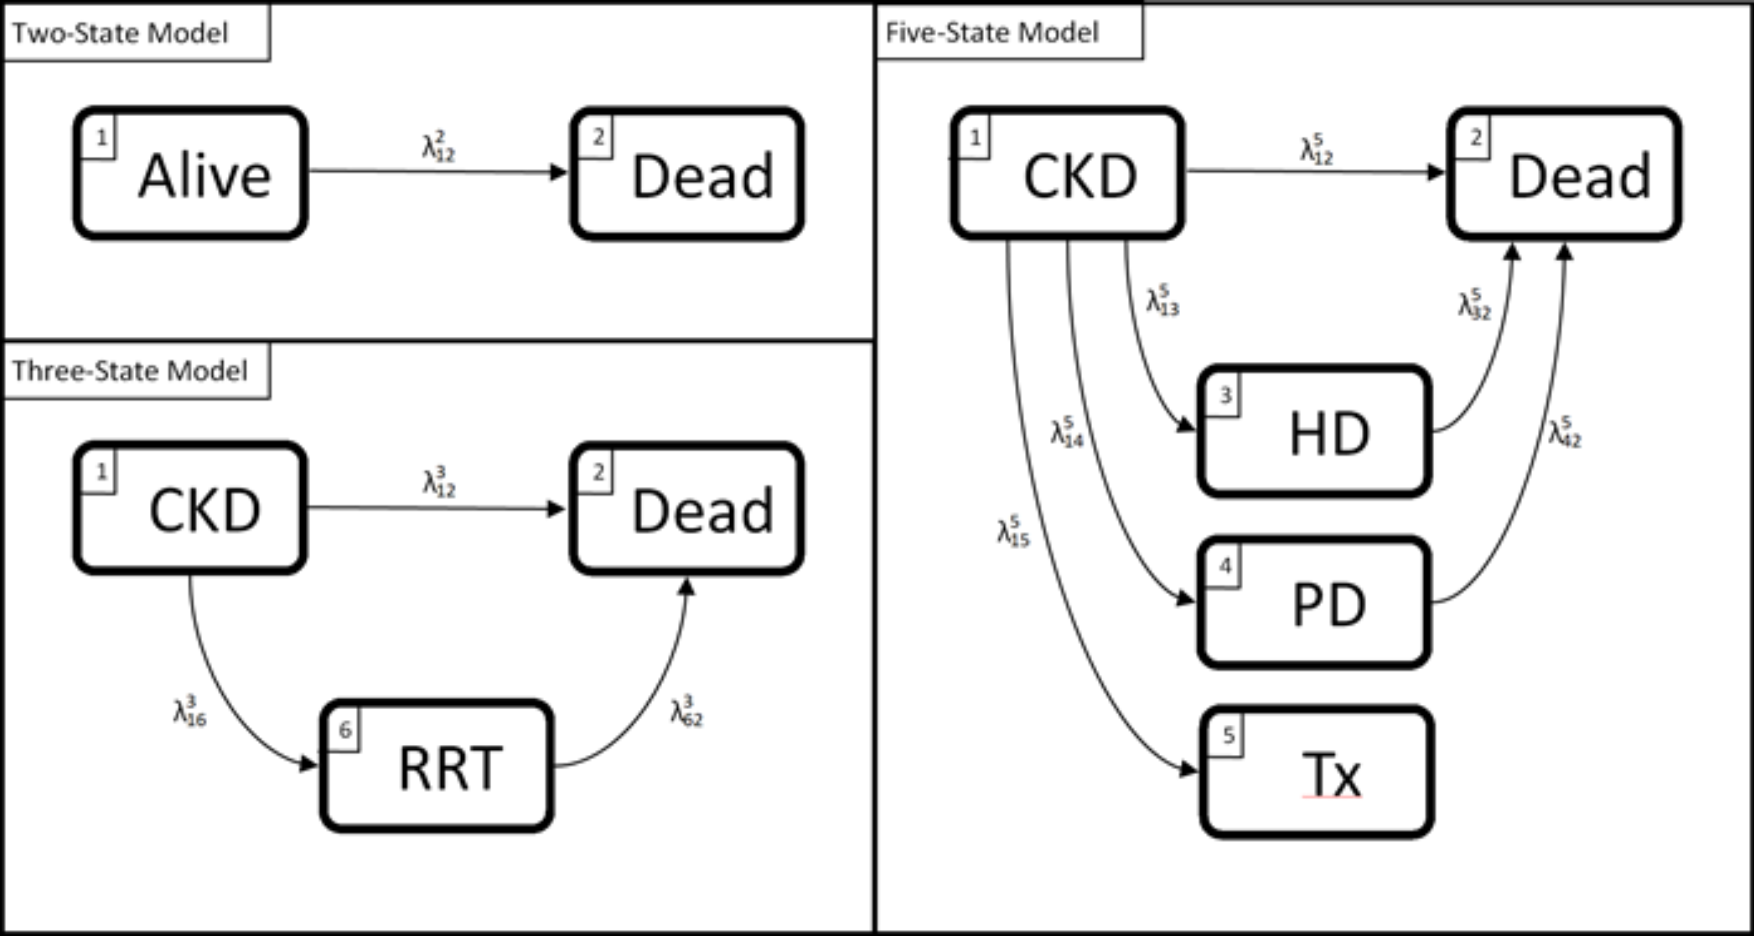
\includegraphics[width=0.9\linewidth]{figure/Dev_Paper_State_Diagrams} 

}

\caption{Diagram of the three models, the states being modelled and relevant transitions}\label{fig:State-Diagram}
\end{figure}
Missing data was handled using multiple imputation (White and Royston \protect\hyperlink{ref-white_imputing_2009}{2009}) using times for all events as imputation covariates. Variables considered as covariates were demographics (sex, age, smoking status and alcohol consumption), comorbidities (congestive cardiac failure (CCF), chronic obstructive pulmonary disease (COPD), prior cerebrovascular accident (CVA), hypertension (HT), diabetes mellitus (DM), ischemic heart disease (IHD), chronic liver disease (LD), prior myocardial infarction (MI), peripheral vascular disease (PVD) and slid tumour (ST)), physical parameters (BMI, blood pressure), blood results (haemoglobin, albumin, corrected calcium and phosphate measures), urine protein creatinine ratio (uPCR) and primary renal diagnosis (grouped as per ERA-EDTA classifications (Venkat-Raman et al. \protect\hyperlink{ref-venkat-raman_new_2012}{2012})). From these variables, uPCR and eGFR Rate of change were also derived (Kovesdy et al. \protect\hyperlink{ref-kovesdy_past_2016}{2016}; Naimark et al. \protect\hyperlink{ref-naimark_past_2016}{2016}) as well as their log transforms and log(Age) and Age\(^2\). For each transition, Backwards-forwards stepwise methods were used to minimise the AIC, allowing different variables to be used for each transition.

\hypertarget{validation}{%
\subsection{Validation}\label{validation}}

Each of the three models were internally validated in the development dataset using bootstrapping to adjust for optimism and then further externally validated in the validation dataset extracted from SERPR (Schomaker and Heumann \protect\hyperlink{ref-schomaker_bootstrap_2018}{2018}). The bootstrapping method was also used for both validations to produce confidence intervals around the performance metric estimates. To assess the performance in low eGFR patients, the models were also validated in subsets of the SKS and SERPR where patients had an eGFR \textless{} 30/ml/min/1.73m\textsuperscript{2}.

Model accuracy was assessed using the Brier Score, discrimination was assessed using the c-statistic and the calibration was assessed using the multi-dimensional intercept and slope-matrix (MA Barrowman, \protect\hyperlink{ref-chap-performance-metrics}{n.d.}). These measures were taken at One-Year, Two-Years and Five-Years after the patient's start dates, and therefore are equivalent to validation measures at that point in time after a prediction has been applied.

Further details of how the models were developed and validated is discussed in the Supplementary materials.

\hypertarget{example}{%
\subsection{Example}\label{example}}

Once the models have been developed, we will apply them to three example patients to demonstrate their use and applicability to the general population. We will provide a direct clinical estimation of these patient outcomes based on years of nephrological experience and compare this with the results presented by our clinical prediction model.

We have chosen three (synthetic) patients to use as examples of the use of our model. Their details can be seen in table \ref{tab:Example-Patient}.
\begin{table}[!h]

\caption{\label{tab:Example-Patient}{\small Details of the Example Patients}}
\centering
\fontsize{7}{9}\selectfont
\begin{tabular}[t]{>{\raggedright\arraybackslash}p{3.5cm}>{\raggedright\arraybackslash}p{3.5cm}>{\raggedright\arraybackslash}p{3.5cm}>{\raggedright\arraybackslash}p{3.5cm}}
\toprule
  & Patient 1 & Patient 2 & Patient 3\\
\midrule
\rowcolor{gray!6}  Age & 20 & 40 & 66\\
Gender & Female & Male & Female\\
\rowcolor{gray!6}  Smoking Status & Non-Smoker & Smoker & Non-Smoker\\
BP & 144/101 & 160/90 & 140/80\\
\rowcolor{gray!6}  Albumin & 39 & 40 & 40\\
\addlinespace
Correct Calcium & 2.3 & 3.0 & 2.6\\
\rowcolor{gray!6}  Haemoglobin & 150 & 100 & 14\\
Phosphate & 0.68 & 2.00 & 0.86\\
\rowcolor{gray!6}  eGFR & 42 & 10 & 51\\
eGFR Previous & 50 (one week ago) & 30 (one year ago) & 70 (one week ago)\\
\addlinespace
\rowcolor{gray!6}  uPCR & 0.30 & 0.20 & 0.01\\
uPCR Previous & 0.80 (one month ago) & 1.20 (one year ago) & 0.06 (one week ago)\\
\rowcolor{gray!6}  Primary Diagnosis & Glomerulonephritis & Tubular Necrosis & Diabetes\\
Comorbities & Chronic Obstructive Pulmonary Disease\newline Liver Disease\newline Solid Tumour &  & Diabetes\newline Chronic Obstructive Pulmonary Disease\newline Hypertension\\
\bottomrule
\end{tabular}
\end{table}
Out three example patients cover a broad range of ages and other covariates. A clinically guided prediction for these patients would assume that Patient 1 has a high chance of proceeding as normal (with little need for RRT), Patient 2 would be recommended to start RRT soon and Patient 3 would be predicted to have a high risk of mortality with or without RRT.

\hypertarget{calculator}{%
\subsection{Calculator}\label{calculator}}

As part of this work, we have also produced an online calculator to allow patients and clinicians to easily estimate outcomes without worrying about the mathematics involved.

All analysis was done in \texttt{R\ 3.6.2} (Team, \protect\hyperlink{ref-r_core_team_r_nodate}{n.d.}) using the various \texttt{tidyverse} packages (Wickham \protect\hyperlink{ref-wickham_tidy_2017}{2017}), as well as the \texttt{mice} (Buuren and Groothuis-Oudshoorn \protect\hyperlink{ref-buuren_mice_2011-1}{2011}), \texttt{flexsurv} (Jackson, \protect\hyperlink{ref-jackson_flexsurv_nodate}{n.d.}), \texttt{nnet} (Ripley and Venables \protect\hyperlink{ref-ripley_package_2016}{2016}) and \texttt{furrr} (Vaughan and Dancho \protect\hyperlink{ref-vaughan_furrr_2018}{2018}) packages. The calculator was produced using the \texttt{shiny} package (Chang et al. \protect\hyperlink{ref-chang_shiny_2020}{2020}).

\hypertarget{results-1}{%
\section{Results}\label{results-1}}

\hypertarget{data-sources-1}{%
\subsection{Data Sources}\label{data-sources-1}}

As seen in table \ref{tab:Table-One}, the Age of the populations had a mean of 64.4 and 65.9 respectively with a very broad range. Due to the inclusion criteria, eGFR were capped at a maximum of 60, and was consistent across populations; however, the rate of change for eGFR was much wider in the SERPR patients than in the SKS, and it was decreasing much faster, on average ( -25 vs 0) . The uPCR measures are presented in our results as g/mmol, rather than the more conventional g/mol, this is to better present results and coefficients of varying magnitudes. Levels of missingness were much higher in the SERPR dataset in most continuous variables.
\begin{table}[!h]

\caption{\label{tab:Table-One}{\small Patient Demographics, Continuous variables are displayed as mean (Inter-Quartile Range), and Categorical/Comorbidity data as number (percent)}}
\centering
\fontsize{7}{9}\selectfont
\begin{tabular}[t]{>{}l>{\ttfamily}l>{\ttfamily}l>{\ttfamily}l>{\ttfamily}l>{\ttfamily}l>{\ttfamily}l}
\toprule
\multicolumn{1}{c}{ } & \multicolumn{3}{c}{SKS} & \multicolumn{3}{c}{SERPR} \\
\cmidrule(l{3pt}r{3pt}){2-4} \cmidrule(l{3pt}r{3pt}){5-7}
Variable & mean/n (IQR/p\%) & missing n (p\%) & range & mean/n (IQR/p\%) & missing n (p\%) & range\\
\midrule
\rowcolor{gray!6}  Age & 64.378 (19.000) & \quad \quad 0 ( 0.00\%) & [ 20.000,\quad 94.000] & 66.064 (17.000) & \quad \quad 0 (\quad 0.00\%) & [\quad 11.000,\quad 98.000]\\
eGFR & 30.369 (22.387) & \quad \quad 0 ( 0.00\%) & [\quad 3.578,\quad 59.966] & 35.647 (20.565) & \quad \quad 0 (\quad 0.00\%) & [ \quad 1.199,\quad 59.994]\\
\rowcolor{gray!6}  eGFR Rate & -0.016 ( 0.294) & 1,278 (42.87\%) & [-19.107,\quad 33.782] & \quad 1.319 (21.897) & \quad \quad 0 (\quad 0.00\%) & [ -28.636,\quad 50.653]\\
SBP & 140.193 (29.000) & \quad 50 ( 1.68\%) & [ 77.000, 220.000] & 145.981 (30.000) & 6,345 ( 82.31\%) & [\quad 82.000, 258.000]\\
\rowcolor{gray!6}  DBP & 74.556 (14.000) & \quad 52 ( 1.74\%) & [ 36.000, 159.000] & 76.742 (17.000) & 6,345 ( 82.31\%) & [\quad 35.000, 128.000]\\
\addlinespace
BMI & 28.848 ( 7.842) & \quad 572 (19.19\%) & [ 13.182,\quad 61.467] & 29.020 ( 6.811) & 7,491 ( 97.17\%) & [\quad 17.073,\quad 52.403]\\
\rowcolor{gray!6}  Albumin & 42.152 ( 5.000) & \quad 60 ( 2.01\%) & [ 12.000,\quad 52.000] & 36.475 ( 6.000) & 3,134 ( 40.65\%) & [ \quad 7.000,\quad 53.000]\\
Calcium & \quad 2.302 ( 0.180) & \quad 68 ( 2.28\%) & [\quad 1.210, \quad 3.660] & \quad 2.407 ( 0.160) & 4,513 ( 58.54\%) & [ \quad 1.455, \quad 3.400]\\
\rowcolor{gray!6}  Haemoglobin & 122.978 (23.000) & \quad 72 ( 2.42\%) & [ 61.000, 195.000] & 109.269 (29.000) & 3,557 ( 46.14\%) & [ \quad 7.100, 208.000]\\
Phosphate & \quad 1.163 ( 0.320) & \quad 87 ( 2.92\%) & [\quad 0.430, \quad 3.710] & \quad 1.194 ( 0.320) & 4,510 ( 58.50\%) & [ \quad 0.320, \quad 4.370]\\
\addlinespace
\rowcolor{gray!6}  uPCR & \quad 0.112 ( 0.103) & \quad 245 ( 8.22\%) & [\quad 0.001, \quad 2.025] & \quad 0.178 ( 0.177) & 7,170 ( 93.01\%) & [ \quad 0.001, \quad 1.943]\\
uPCR Rate & -0.096 ( 0.188) & 1,777 (59.61\%) & [-70.727,\quad 28.199] & \quad 4.621 ( 0.905) & 7,495 ( 97.22\%) & [-176.200, 952.812]\\
\rowcolor{gray!6}  Gender: &  & \quad \quad 0 ( 0.00\%) &  &  & \quad \quad 0 (\quad 0.00\%) & \\
Male & \quad 1,865 (62.56\%) &  &  & \quad 3,885 (50.40\%) &  & \\
\rowcolor{gray!6}  Female & \quad 1,116 (37.44\%) &  &  & \quad 3,824 (49.60\%) &  & \\
\addlinespace
Ethnicity: &  & \quad \quad 0 ( 0.00\%) &  &  & 7,009 ( 90.92\%) & \\
\rowcolor{gray!6}  White & \quad 2,875 (96.44\%) &  &  & \quad \quad 679 ( 8.81\%) &  & \\
Asian & \quad \quad 75 ( 2.52\%) &  &  & \quad \quad 12 ( 0.16\%) &  & \\
\rowcolor{gray!6}  Black & \quad \quad 21 ( 0.70\%) &  &  & \quad \quad \quad 7 ( 0.09\%) &  & \\
Other & \quad \quad 10 ( 0.34\%) &  &  & \quad \quad \quad 2 ( 0.03\%) &  & \\
\addlinespace
\rowcolor{gray!6}  SmokingStatus: &  & \quad 42 ( 1.41\%) &  &  & 7,709 (100.00\%) & \\
Former & \quad 1,535 (51.49\%) &  &  & \quad \quad \quad 0 ( 0.00\%) &  & \\
\rowcolor{gray!6}  Non-Smoker & \quad \quad 979 (32.84\%) &  &  & \quad \quad \quad 0 ( 0.00\%) &  & \\
Smoker & \quad \quad 379 (12.71\%) &  &  & \quad \quad \quad 0 ( 0.00\%) &  & \\
\rowcolor{gray!6}  Former 3Y & \quad \quad 46 ( 1.54\%) &  &  & \quad \quad \quad 0 ( 0.00\%) &  & \\
\addlinespace
DiagGroup: &  & \quad 567 (19.02\%) &  &  & 6,640 ( 86.13\%) & \\
\rowcolor{gray!6}  Systemic diseases affecting the kidney & \quad 1,304 (43.74\%) &  &  & \quad \quad 316 ( 4.10\%) &  & \\
Glomerular disease & \quad \quad 442 (14.83\%) &  &  & \quad \quad 278 ( 3.61\%) &  & \\
\rowcolor{gray!6}  Tubulointerstitial disease & \quad \quad 268 ( 8.99\%) &  &  & \quad \quad 173 ( 2.24\%) &  & \\
Miscellaneous renal disorders & \quad \quad 227 ( 7.61\%) &  &  & \quad \quad 198 ( 2.57\%) &  & \\
\addlinespace
\rowcolor{gray!6}  Familial / hereditary nephropathies & \quad \quad 173 ( 5.80\%) &  &  & \quad \quad 104 ( 1.35\%) &  & \\
Diabetes (DM) & \quad \quad 992 (33.32\%) & \quad \quad 4 ( 0.13\%) &  & \quad 1,535 (19.91\%) & \quad \quad 0 (\quad 0.00\%) & \\
\rowcolor{gray!6}  Congestive Cardiac Failure (CCF) & \quad 2,414 (81.09\%) & \quad \quad 4 ( 0.13\%) &  & \quad \quad 408 ( 5.29\%) & \quad \quad 0 (\quad 0.00\%) & \\
Prior Myocardial Infarction (MI) & \quad 2,492 (83.71\%) & \quad \quad 4 ( 0.13\%) &  & \quad \quad 556 ( 7.21\%) & \quad \quad 0 (\quad 0.00\%) & \\
\rowcolor{gray!6}  Ischemic Heart Disease (IHD) & \quad 2,393 (80.38\%) & \quad \quad 4 ( 0.13\%) &  & \quad \quad 863 (11.19\%) & \quad \quad 0 (\quad 0.00\%) & \\
\addlinespace
Peripheral Vascular Disease (PVA) & \quad 2,485 (83.47\%) & \quad \quad 4 ( 0.13\%) &  & \quad \quad 376 ( 4.88\%) & \quad \quad 0 (\quad 0.00\%) & \\
\rowcolor{gray!6}  Prior Cerebrovascular Accident (CVA) & \quad 2,727 (91.60\%) & \quad \quad 4 ( 0.13\%) &  & \quad \quad 186 ( 2.41\%) & \quad \quad 0 (\quad 0.00\%) & \\
Chronic Obstructive Pulmonary Disease (COPD) & \quad 2,411 (80.99\%) & \quad \quad 4 ( 0.13\%) &  & \quad \quad \quad 0 ( \quad \quad \%) & 7,709 (100.00\%) & \\
\rowcolor{gray!6}  Chronic Liver Disease (LD) & \quad 2,891 (97.11\%) & \quad \quad 4 ( 0.13\%) &  & \quad \quad \quad 0 ( \quad \quad \%) & 7,709 (100.00\%) & \\
Prior Solid Tumour (ST) & \quad 2,570 (86.33\%) & \quad \quad 4 ( 0.13\%) &  & \quad \quad \quad 0 ( \quad \quad \%) & 7,709 (100.00\%) & \\
\addlinespace
\rowcolor{gray!6}  Hypertension (HT) & \quad 2,546 (91.48\%) & \quad 198 ( 6.64\%) &  & \quad 3,114 (40.39\%) & \quad \quad 0 (\quad 0.00\%) & \\
\bottomrule
\end{tabular}
\end{table}
Table \ref{tab:Table-One} also shows a breakdown of the categorical variables across the populations. In the development population, crude proportions of males were numerically higher than females whereas in the validation population the proportions are much more matched (62.6\% male vs 50.4\% male). Most patients were white in the SKS dataset, and ethnicity has extremely high missingness in SERPR, which also contributed to its omission from the model.

Overall, there were high levels of comorbidities within the SKS population, but these levels were much lower in the SERPR population.

The median date for the date of death was 3.9 years in the SKS population and 4.9 years in the SERPR population. The median date for transition to RRT was 2.2 years and 1.5 years (in SKS and SERPR respectively). In SKS, transitions to HD happened 6 months later than PD, and in SERPR it was 3.6 months. The Maximum followup time in SKS was 15.0 years and in SERPR it was 10.1 years. This information can be seen in table \ref{tab:Event-Median2}.
\begin{table}[!h]

\caption{\label{tab:Event-Median2}{\small Event times for the two populations presented as Number of Events ~ Median (Inter-Quartile Range) [Max]}}
\centering
\fontsize{7}{9}\selectfont
\begin{tabular}[t]{>{}r>{}r>{}r>{\ttfamily}r>{\ttfamily}r>{\ttfamily}r>{\ttfamily}r>{\ttfamily}r>{\ttfamily}r>{\ttfamily}r>{\ttfamily}r}
\toprule
\multicolumn{3}{c}{Transition} & \multicolumn{4}{c}{SKS} & \multicolumn{4}{c}{SERPR} \\
\cmidrule(l{3pt}r{3pt}){1-3} \cmidrule(l{3pt}r{3pt}){4-7} \cmidrule(l{3pt}r{3pt}){8-11}
Model & From & To & n & median & IQR & max & n & median & IQR & max\\
\midrule
\rowcolor{gray!6}  Two & Alive & Dead & 1,427 & 4.0 y & 4.3 y & 15.0 y & 3,010 & 4.8 y & 3.3 y & 10.1 y\\
Three & CKD & Dead & 1,125 & 3.5 y & 4.2 y & 15.0 y & 2,568 & 4.7 y & 3.3 y & 10.1 y\\
\rowcolor{gray!6}   &  & RRT & \quad 680 & 2.5 y & 3.4 y & 14.2 y & 1,125 & 3.8 y & 3.9 y & 10.1 y\\
 & RRT & Dead & \quad 302 & 2.2 y & 3.3 y & 13.5 y & \quad 442 & 1.6 y & 2.5 y & 9.2 y\\
\rowcolor{gray!6}  Five & CKD & Dead & 1,125 & 3.5 y & 4.2 y & 15.0 y & 2,568 & 4.7 y & 3.3 y & 10.1 y\\
\addlinespace
 &  & HD & \quad 344 & 2.6 y & 3.5 y & 14.2 y & \quad 882 & 3.7 y & 3.8 y & 10.1 y\\
\rowcolor{gray!6}   &  & PD & \quad 229 & 2.0 y & 2.9 y & 12.9 y & \quad 149 & 3.5 y & 4.1 y & 9.5 y\\
 &  & Tx & \quad 107 & 3.2 y & 2.7 y & 12.1 y & \quad 94 & 5.0 y & 4.4 y & 9.8 y\\
\rowcolor{gray!6}   & HD & Dead & \quad 185 & 2.1 y & 3.3 y & 11.8 y & \quad 394 & 1.6 y & 2.5 y & 9.2 y\\
 & PD & Dead & \quad 107 & 2.4 y & 3.2 y & 11.8 y & \quad 47 & 2.1 y & 2.3 y & 8.5 y\\
\bottomrule
\end{tabular}
\end{table}
\hypertarget{development}{%
\subsection{Development}\label{development}}

Here we present the proportional hazards results for the Three-State Model. The full model description, including proportional and baseline hazards can be found in the Supplementary Materials. Older patients are predicted to be likely to transition to RRT. Increased rates of decline of eGFR were associated with the transition from CKD to RRT. The full results are shown in table \ref{tab:PH-Three}.
\begin{table}[!h]

\caption{\label{tab:PH-Three}{\small Proportional Hazards for each transition in the Three-State Model}}
\centering
\fontsize{7}{9}\selectfont
\begin{tabular}[t]{>{\raggedright\arraybackslash}p{30em}>{\ttfamily\raggedleft\arraybackslash}p{43em}>{\ttfamily\raggedleft\arraybackslash}p{43em}>{\ttfamily\raggedleft\arraybackslash}p{43em}}
\toprule
  & CKD to Dead & CKD to RRT & RRT to Dead\\
\midrule
\rowcolor{gray!6}  \addlinespace[0.3em]
\multicolumn{4}{l}{\textbf{Age}}\\
\hspace{1em}(Age-60) & 0.162 (\quad -0.051, \quad 0.375) & -0.041 (\quad -0.051,\quad -0.032) & 0.063 ( \quad 0.051, \quad 0.076)\\
\hspace{1em}(Age-60)\textsuperscript{} & -0.001 (\quad -0.003, \quad 0.001) & 0.000 (\quad -0.001, \quad 0.000) & \\
\rowcolor{gray!6}  \hspace{1em}log(Age) & -5.725 ( -17.969, \quad 6.519) &  & \\
\addlinespace[0.3em]
\multicolumn{4}{l}{\textbf{eGFR}}\\
\hspace{1em}eGFR & -0.013 (\quad -0.020,\quad -0.007) & -0.096 (\quad -0.109,\quad -0.083) & 0.012 (\quad -0.002, \quad 0.026)\\
\rowcolor{gray!6}  \hspace{1em}eGFR Rate &  & 0.055 (\quad -0.021, \quad 0.131) & -0.056 (\quad -0.364, \quad 0.251)\\
\hspace{1em}log(eGFR Rate) & 0.043 (\quad -0.125, \quad 0.211) &  & 0.228 (\quad -0.770, \quad 1.226)\\
\rowcolor{gray!6}  \addlinespace[0.3em]
\multicolumn{4}{l}{\textbf{uPCR}}\\
\hspace{1em}uPCR & 0.125 (\quad -0.318, \quad 0.569) & 0.700 ( \quad 0.113, \quad 1.288) & -0.108 (\quad -0.736, \quad 0.519)\\
\hspace{1em}uPCR Rate &  & -0.020 (\quad -0.045, \quad 0.005) & 0.037 (\quad -0.063, \quad 0.136)\\
\rowcolor{gray!6}  \hspace{1em}log(uPCR Rate) &  & 0.218 (\quad -0.311, \quad 0.748) & -0.198 (\quad -0.534, \quad 0.137)\\
\addlinespace[0.3em]
\multicolumn{4}{l}{\textbf{Measures}}\\
\hspace{1em}SBP & -0.001 (\quad -0.005, \quad 0.002) & 0.005 (\quad -0.001, \quad 0.011) & \\
\rowcolor{gray!6}  \hspace{1em}DBP & 0.007 ( \quad 0.000, \quad 0.013) & 0.007 (\quad -0.002, \quad 0.016) & \\
\hspace{1em}BMI &  &  & \\
\rowcolor{gray!6}  \hspace{1em}Albumin & -0.045 (\quad -0.065,\quad -0.024) & -0.032 (\quad -0.060,\quad -0.005) & -0.045 (\quad -0.080,\quad -0.010)\\
\hspace{1em}Corrected Calcium & 0.280 (\quad -0.192, \quad 0.753) & -0.515 (\quad -1.208, \quad 0.177) & \\
\rowcolor{gray!6}  \hspace{1em}Haemoglobin & -0.013 (\quad -0.018,\quad -0.008) & -0.005 (\quad -0.012, \quad 0.002) & -0.006 (\quad -0.015, \quad 0.004)\\
\hspace{1em}Phosphate & 0.512 ( \quad 0.133, \quad 0.891) & 0.870 (\quad -0.060, \quad 1.800) & \\
\rowcolor{gray!6}  \addlinespace[0.3em]
\multicolumn{4}{l}{\textbf{Gender}}\\
\hspace{1em}Female & -0.236 (\quad -0.371,\quad -0.100) & -0.278 (\quad -0.456,\quad -0.100) & \\
\addlinespace[0.3em]
\multicolumn{4}{l}{\textbf{Smoking Status}}\\
\hspace{1em}Former (3 years+) & -0.213 (\quad -0.879, \quad 0.453) & -0.134 (\quad -0.758, \quad 0.490) & -0.282 (\quad -1.083, \quad 0.519)\\
\rowcolor{gray!6}  \hspace{1em}Non-Smoker & -0.198 (\quad -0.345,\quad -0.051) & -0.162 (\quad -0.364, \quad 0.040) & -0.295 (\quad -0.599, \quad 0.010)\\
\hspace{1em}Smoker & 0.356 ( \quad 0.161, \quad 0.552) & 0.176 (\quad -0.077, \quad 0.428) & 0.387 ( \quad 0.069, \quad 0.706)\\
\rowcolor{gray!6}  \addlinespace[0.3em]
\multicolumn{4}{l}{\textbf{Primary Renal Diagnosis}}\\
\hspace{1em}Familial / hereditary nephropathies & -0.424 (\quad -0.855, \quad 0.006) & 1.029 ( \quad 0.721, \quad 1.338) & -0.563 (\quad -1.085,\quad -0.040)\\
\hspace{1em}Glomerular disease & -0.395 (\quad -0.636,\quad -0.154) & -0.166 (\quad -0.465, \quad 0.134) & -0.489 (\quad -0.884,\quad -0.094)\\
\rowcolor{gray!6}  \hspace{1em}Miscellaneous renal disorders & -0.263 (\quad -0.506,\quad -0.021) & -0.649 (\quad -1.143,\quad -0.155) & 0.033 (\quad -0.554, \quad 0.620)\\
\hspace{1em}Tubulointerstitial disease & -0.463 (\quad -0.742,\quad -0.185) & -0.266 (\quad -0.577, \quad 0.046) & -0.311 (\quad -0.803, \quad 0.182)\\
\rowcolor{gray!6}  \addlinespace[0.3em]
\multicolumn{4}{l}{\textbf{Comorbidity}}\\
\hspace{1em}DM & 0.122 (\quad -0.011, \quad 0.255) & 0.142 (\quad -0.075, \quad 0.359) & 0.200 (\quad -0.096, \quad 0.497)\\
\hspace{1em}CCF & -0.395 (\quad -0.536,\quad -0.254) &  & -0.300 (\quad -0.597,\quad -0.003)\\
\rowcolor{gray!6}  \hspace{1em}MI & -0.246 (\quad -0.398,\quad -0.095) & 0.234 (\quad -0.062, \quad 0.530) & 0.187 (\quad -0.199, \quad 0.572)\\
\hspace{1em}IHD & 0.102 (\quad -0.041, \quad 0.246) & -0.077 (\quad -0.334, \quad 0.179) & -0.098 (\quad -0.424, \quad 0.228)\\
\rowcolor{gray!6}  \hspace{1em}PVD & -0.249 (\quad -0.395,\quad -0.103) & -0.169 (\quad -0.406, \quad 0.068) & -0.183 (\quad -0.493, \quad 0.126)\\
\hspace{1em}CVA & -0.071 (\quad -0.253, \quad 0.111) &  & -0.168 (\quad -0.577, \quad 0.241)\\
\rowcolor{gray!6}  \hspace{1em}COPD & -0.290 (\quad -0.433,\quad -0.146) &  & \\
\hspace{1em}LD & -0.170 (\quad -0.579, \quad 0.239) & -0.317 (\quad -0.732, \quad 0.098) & -0.270 (\quad -0.859, \quad 0.318)\\
\rowcolor{gray!6}  \hspace{1em}ST & -0.274 (\quad -0.431,\quad -0.118) & -0.181 (\quad -0.516, \quad 0.153) & -0.278 (\quad -0.612, \quad 0.056)\\
\hspace{1em}HT &  & 0.275 (\quad -0.177, \quad 0.726) & -0.416 (\quad -1.105, \quad 0.272)\\
\bottomrule
\end{tabular}
\end{table}
Female patients are predicted to be more likely to remain in the CKD state than Males, or to remain in the RRT state once there. Smokers were predicted as more likely than Non-/Former Smokers to undergo any transition, apart from CKD to Tx. Blood results had associations with all transitions in some way, and disease etiology were strongly associated with the transitions giving a wide range of predictions.

\hypertarget{validation-1}{%
\subsection{Validation}\label{validation-1}}

Table \ref{tab:IV-Three} shows the results from the internal validation in the Three-State Model. Performance was overall slightly better in patients in the \textless60 eGFR group than in the \textless30 eGFR group. All measures degraded over time, but the average scores remained strong.
\begin{table}[!h]

\caption{\label{tab:IV-Three}{\small Internal Validation of the Three-State Model, results presented as Estimate (95\% CI, where possible)}}
\centering
\fontsize{7}{9}\selectfont
\begin{tabular}[t]{>{}l>{}l>{\ttfamily}r>{\ttfamily}r>{\ttfamily}r>{\ttfamily}r}
\toprule
Predicting & eGFR & One Year & Two Year & Five Year & Average\\
\midrule
\rowcolor{gray!6}  \addlinespace[0.3em]
\multicolumn{6}{l}{\textbf{Brier}}\\
\hspace{1em}Three & < 60 & 0.74 ( 0.74,\quad 0.75) & 0.68 ( 0.68,\quad 0.69) & 0.64 ( 0.64,\quad 0.65) & 0.67 ( 0.67,\quad 0.68)\\
\hspace{1em}Three & < 30 & 0.75 ( 0.74,\quad 0.75) & 0.73 ( 0.73,\quad 0.73) & 0.68 ( 0.67,\quad 0.68) & 0.68 ( 0.67,\quad 0.68)\\
\rowcolor{gray!6}  \hspace{1em}Two & < 60 & 0.75 ( 0.75,\quad 0.75) & 0.75 ( 0.75,\quad 0.76) & 0.67 ( 0.67,\quad 0.67) & 0.67 ( 0.67,\quad 0.68)\\
\hspace{1em}Two & < 30 & 0.71 ( 0.71,\quad 0.72) & 0.72 ( 0.72,\quad 0.73) & 0.65 ( 0.65,\quad 0.66) & 0.67 ( 0.67,\quad 0.68)\\
\rowcolor{gray!6}  \addlinespace[0.3em]
\multicolumn{6}{l}{\textbf{c-statistic}}\\
\hspace{1em}Three & < 60 & 0.87 ( 0.87,\quad 0.87) & 0.84 ( 0.84,\quad 0.85) & 0.84 ( 0.84,\quad 0.84) & 0.83 ( 0.83,\quad 0.84)\\
\hspace{1em}Three & < 30 & 0.87 ( 0.86,\quad 0.87) & 0.84 ( 0.84,\quad 0.84) & 0.84 ( 0.84,\quad 0.84) & 0.83 ( 0.83,\quad 0.84)\\
\rowcolor{gray!6}  \hspace{1em}Two & < 60 & 0.86 ( 0.86,\quad 0.86) & 0.86 ( 0.86,\quad 0.86) & 0.83 ( 0.83,\quad 0.84) & 0.83 ( 0.83,\quad 0.84)\\
\hspace{1em}Two & < 30 & 0.86 ( 0.85,\quad 0.86) & 0.86 ( 0.85,\quad 0.86) & 0.85 ( 0.85,\quad 0.85) & 0.84 ( 0.83,\quad 0.84)\\
\rowcolor{gray!6}  \addlinespace[0.3em]
\multicolumn{6}{l}{\textbf{Intercept}}\\
\hspace{1em}Three & < 60 & \makecell[r]{-0.00 (-0.00,\quad 0.00)\\\quad 0.00 ( 0.00,\quad 0.01)\\\quad 0.00 ( 0.00,\quad 0.00)} & \makecell[r]{0.00 (-0.00,\quad 0.00)\\ -0.01 (-0.02, -0.01)\\\quad 0.00 ( 0.00,\quad 0.00)} & \makecell[r]{-0.02 (-0.02, -0.01)\\ -0.01 (-0.02, -0.01)\\ -0.00 (-0.01, -0.00)} & \makecell[r]{0.00 ( 0.00,\quad 0.00)\\\quad 0.00 (-0.00,\quad 0.00)\\\quad 0.00 (-0.00,\quad 0.00)}\\
\hspace{1em}Three & < 30 & \makecell[r]{-0.01 (-0.01, -0.01)\\ -0.00 (-0.00, -0.00)\\\quad 0.00 (-0.00,\quad 0.00)} & \makecell[r]{0.00 (-0.00,\quad 0.00)\\ -0.01 (-0.01, -0.00)\\\quad 0.03 ( 0.02,\quad 0.03)} & \makecell[r]{-0.02 (-0.02, -0.01)\\\quad 0.00 (-0.00,\quad 0.00)\\ -0.00 (-0.01, -0.00)} & \makecell[r]{0.00 (-0.00,\quad 0.00)\\\quad 0.00 (-0.00,\quad 0.00)\\\quad 0.00 (-0.00,\quad 0.00)}\\
\rowcolor{gray!6}  \hspace{1em}Two & < 60 & -0.00 (-0.01, -0.00) & 0.02 ( 0.01,\quad 0.02) & 0.00 (-0.00,\quad 0.00) & -0.00 (-0.00,\quad 0.00)\\
\hspace{1em}Two & < 30 & -0.00 (-0.00,\quad 0.00) & -0.04 (-0.04, -0.04) & 0.00 ( 0.00,\quad 0.01) & -0.00 (-0.00,\quad 0.00)\\
\rowcolor{gray!6}  \addlinespace[0.3em]
\multicolumn{6}{l}{\textbf{Slope}}\\
\hspace{1em}Three & < 60 & \makecell[r]{\emph{1.25},\quad 0.00,\quad 0.04\\ -0.03,\quad \emph{1.10}, -0.00\\ -0.00,\quad 0.01,\quad \emph{1.16}} & \makecell[r]{\emph{1.17}, -0.06,\quad 0.01\\\quad 0.03,\quad \emph{1.25}, -0.01\\ -0.01,\quad 0.01,\quad \emph{1.37}} & \makecell[r]{\emph{1.21}, -0.02, -0.01\\\quad 0.01,\quad \emph{1.44}, -0.04\\ -0.02,\quad 0.02,\quad \emph{1.27}} & \makecell[r]{\emph{1.32}, -0.01,\quad 0.00\\ -0.00,\quad \emph{1.37}, -0.01\\ -0.00,\quad 0.00,\quad \emph{1.33}}\\
\hspace{1em}Three & < 30 & \makecell[r]{\emph{1.21},\quad 0.02,\quad 0.07\\ -0.04,\quad \emph{1.24},\quad 0.07\\\quad 0.01,\quad 0.01,\quad \emph{1.16}} & \makecell[r]{\emph{1.36}, -0.00, -0.01\\\quad 0.00,\quad \emph{1.31},\quad 0.03\\ -0.02, -0.00,\quad \emph{1.26}} & \makecell[r]{\emph{1.35}, -0.04, -0.01\\\quad 0.04,\quad \emph{1.33},\quad 0.04\\\quad 0.04, -0.02,\quad \emph{1.34}} & \makecell[r]{\emph{1.31},\quad 0.00,\quad 0.00\\ -0.01,\quad \emph{1.33},\quad 0.01\\ -0.00,\quad 0.00,\quad \emph{1.35}}\\
\rowcolor{gray!6}  \hspace{1em}Two & < 60 & \emph{1.21} & \emph{1.28} & \emph{1.27} & \emph{1.31}\\
\hspace{1em}Two & < 30 & \emph{1.05} & \emph{1.21} & \emph{1.21} & \emph{1.34}\\
\bottomrule
\end{tabular}
\end{table}
Table \ref{tab:EV-Three} shows the results from the external validation in the Three-State Model.
\begin{table}[!h]

\caption{\label{tab:EV-Three}{\small External Validation of the Three-State Model, results presented as Estimate (95\% CI, where possible)}}
\centering
\fontsize{7}{9}\selectfont
\begin{tabular}[t]{>{}l>{}l>{\ttfamily}r>{\ttfamily}r>{\ttfamily}r>{\ttfamily}r}
\toprule
Predicting & eGFR & One Year & Two Year & Five Year & Average\\
\midrule
\rowcolor{gray!6}  \addlinespace[0.3em]
\multicolumn{6}{l}{\textbf{Brier}}\\
\hspace{1em}Three & < 60 & 0.69 ( 0.68,\quad 0.69) & 0.70 ( 0.69,\quad 0.70) & 0.61 ( 0.60,\quad 0.61) & 0.62 ( 0.62,\quad 0.63)\\
\hspace{1em}Three & < 30 & 0.68 ( 0.67,\quad 0.68) & 0.72 ( 0.71,\quad 0.72) & 0.65 ( 0.64,\quad 0.65) & 0.63 ( 0.62,\quad 0.63)\\
\rowcolor{gray!6}  \hspace{1em}Two & < 60 & 0.67 ( 0.67,\quad 0.67) & 0.70 ( 0.69,\quad 0.70) & 0.63 ( 0.63,\quad 0.63) & 0.62 ( 0.62,\quad 0.63)\\
\hspace{1em}Two & < 30 & 0.66 ( 0.66,\quad 0.67) & 0.70 ( 0.70,\quad 0.70) & 0.65 ( 0.65,\quad 0.66) & 0.63 ( 0.62,\quad 0.63)\\
\rowcolor{gray!6}  \addlinespace[0.3em]
\multicolumn{6}{l}{\textbf{c-statistic}}\\
\hspace{1em}Three & < 60 & 0.82 ( 0.82,\quad 0.82) & 0.83 ( 0.83,\quad 0.83) & 0.79 ( 0.79,\quad 0.79) & 0.81 ( 0.80,\quad 0.81)\\
\hspace{1em}Three & < 30 & 0.85 ( 0.84,\quad 0.85) & 0.84 ( 0.84,\quad 0.84) & 0.83 ( 0.83,\quad 0.83) & 0.81 ( 0.81,\quad 0.81)\\
\rowcolor{gray!6}  \hspace{1em}Two & < 60 & 0.85 ( 0.85,\quad 0.86) & 0.84 ( 0.84,\quad 0.85) & 0.80 ( 0.80,\quad 0.80) & 0.81 ( 0.80,\quad 0.81)\\
\hspace{1em}Two & < 30 & 0.83 ( 0.83,\quad 0.83) & 0.82 ( 0.82,\quad 0.82) & 0.80 ( 0.80,\quad 0.81) & 0.81 ( 0.81,\quad 0.81)\\
\rowcolor{gray!6}  \addlinespace[0.3em]
\multicolumn{6}{l}{\textbf{Intercept}}\\
\hspace{1em}Three & < 60 & \makecell[r]{0.00 (-0.00,\quad 0.00)\\\quad 0.00 ( 0.00,\quad 0.00)\\ -0.00 (-0.00, -0.00)} & \makecell[r]{0.01 ( 0.01,\quad 0.02)\\ -0.01 (-0.01, -0.00)\\\quad 0.00 ( 0.00,\quad 0.01)} & \makecell[r]{0.05 ( 0.04,\quad 0.05)\\\quad 0.01 ( 0.00,\quad 0.01)\\\quad 0.00 ( 0.00,\quad 0.00)} & \makecell[r]{-0.00 (-0.00,\quad 0.00)\\ -0.00 (-0.00,\quad 0.00)\\\quad 0.00 ( 0.00,\quad 0.01)}\\
\hspace{1em}Three & < 30 & \makecell[r]{0.04 ( 0.04,\quad 0.05)\\\quad 0.01 ( 0.00,\quad 0.01)\\\quad 0.00 ( 0.00,\quad 0.01)} & \makecell[r]{0.02 ( 0.01,\quad 0.02)\\ -0.00 (-0.00,\quad 0.00)\\\quad 0.01 ( 0.01,\quad 0.02)} & \makecell[r]{0.01 ( 0.01,\quad 0.01)\\ -0.00 (-0.00,\quad 0.00)\\\quad 0.00 ( 0.00,\quad 0.01)} & \makecell[r]{0.00 (-0.00,\quad 0.00)\\\quad 0.00 (-0.00,\quad 0.00)\\ -0.00 (-0.00,\quad 0.00)}\\
\rowcolor{gray!6}  \hspace{1em}Two & < 60 & 0.00 (-0.00,\quad 0.00) & -0.05 (-0.05, -0.04) & 0.01 ( 0.01,\quad 0.02) & -0.00 (-0.00,\quad 0.00)\\
\hspace{1em}Two & < 30 & 0.02 ( 0.01,\quad 0.02) & -0.00 (-0.00,\quad 0.00) & 0.01 ( 0.00,\quad 0.01) & -0.00 (-0.00,\quad 0.00)\\
\rowcolor{gray!6}  \addlinespace[0.3em]
\multicolumn{6}{l}{\textbf{Slope}}\\
\hspace{1em}Three & < 60 & \makecell[r]{\emph{1.35}, -0.04,\quad 0.04\\\quad 0.06,\quad \emph{1.49}, -0.03\\\quad 0.01,\quad 0.00,\quad \emph{1.25}} & \makecell[r]{\emph{1.13}, -0.00,\quad 0.08\\ -0.02,\quad \emph{1.31},\quad 0.01\\ -0.03,\quad 0.01,\quad \emph{1.39}} & \makecell[r]{\emph{1.45}, -0.02,\quad 0.03\\\quad 0.03,\quad \emph{1.73},\quad 0.03\\\quad 0.04, -0.00,\quad \emph{1.47}} & \makecell[r]{\emph{1.54},\quad 0.00, -0.00\\\quad 0.01,\quad \emph{1.52},\quad 0.00\\ -0.00,\quad 0.00,\quad \emph{1.54}}\\
\hspace{1em}Three & < 30 & \makecell[r]{\emph{1.23},\quad 0.03,\quad 0.00\\ -0.05,\quad \emph{1.20}, -0.04\\ -0.00, -0.00,\quad \emph{1.37}} & \makecell[r]{\emph{0.99}, -0.01, -0.00\\\quad 0.04,\quad \emph{1.34}, -0.03\\\quad 0.00,\quad 0.01,\quad \emph{1.46}} & \makecell[r]{\emph{1.56},\quad 0.00,\quad 0.00\\ -0.05,\quad \emph{1.49},\quad 0.03\\\quad 0.03,\quad 0.01,\quad \emph{1.63}} & \makecell[r]{\emph{1.62}, -0.01,\quad 0.01\\ -0.00,\quad \emph{1.53},\quad 0.01\\\quad 0.00, -0.00,\quad \emph{1.58}}\\
\rowcolor{gray!6}  \hspace{1em}Two & < 60 & \emph{1.28} & \emph{1.26} & \emph{1.64} & \emph{1.51}\\
\hspace{1em}Two & < 30 & \emph{1.18} & \emph{1.25} & \emph{1.57} & \emph{1.59}\\
\bottomrule
\end{tabular}
\end{table}
\hypertarget{example-1}{%
\subsection{Example}\label{example-1}}

The example patients seen in Table \ref{tab:Example-Patient} were passed through our Three-State prediction model and the results for all time-points are shown in figure \ref{fig:Example-Predictions-trend}. The prognosis for all three patients were very different. Patient 1 (20 year old) had a very high probability of survival, with only an 16\% chance of mortality by year 10 and 0\% chance of commencing RRT. Patient 2 (40 year old) was predicted almost 90\% chance of starting RRT, and over 70\% chance of dying overall (either with or without RR). Patient 3 (66 year old) had a fast acceleration towards high mortality, after 1 year from the recorded measurements, they had more than 50\% chance of dying, and after 2 years that probability rises to over 85\% with no chance of RRT.
\begin{figure}

{\centering 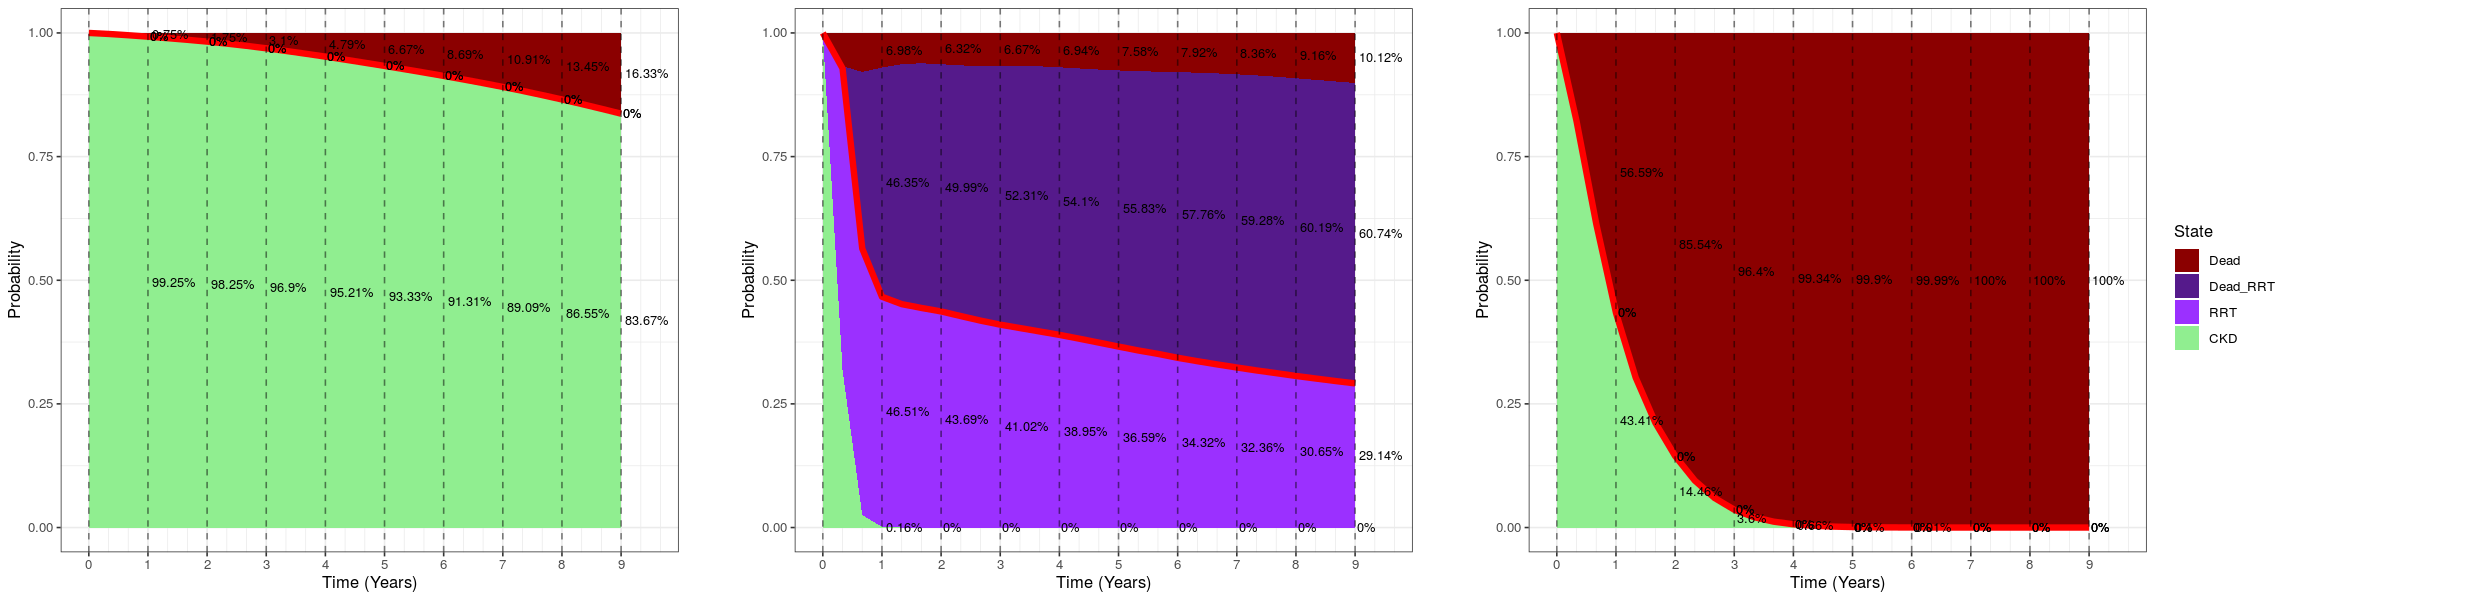
\includegraphics[width=1\linewidth]{figure/Dev_Paper_Example} 

}

\caption{Results of Example Patients}\label{fig:Example-Predictions-trend}
\end{figure}
\hypertarget{calculator-1}{%
\subsection{Calculator}\label{calculator-1}}

The calculator is available online here:

\url{https://michael-barrowman.shinyapps.io/MSCPM_for_CKD_Patients/}.

\hypertarget{discussion}{%
\section{Discussion}\label{discussion}}

We have used data provided by SKS to develop a Multi-State Clinical Prediction Model and then validated this model within the SKS and SERPR datasets. Within our Models, the cause of a patient's renal disease had the widest effect on patient outcomes meaning that outcomes are highly dependent on ERA-EDTA classification of the diagnosis. Most groupings resulted in a lowered hazard of death and an increased hazard of RRT compared to the baseline of Systemic diseases.

Models performed well in model validation with the Three-State Model slightly out performing the other two models in calibration and overall predictive ability, however the Five-State model performed marginally better in terms of discriminative ability. Both Multi-State Models outperformed the Two-State (Traditional) Model.

The application of a Multi-state clinical prediction model to this field is novel and gives a powerful tool for providing individualised predictions of different outcomes at a wide range of time points. The model can also be used to estimate an expected amount of time that a patient will be on RRT The general inclusion criteria for the development dataset, and the wide range of patient ages and measurements allows for the model to be applied to a broad spectrum of patients.

Although the inclusion criteria for SKS were broad, the demographics of the local area resulted in homogeneity of ethnicity, which may create a limitation to the applicability of our model. The Renal Department at SRFT is a tertiary care facility for CKD sufferers and is well renowned for its capabilities of care meaning that it is likely to attract less-healthy patients from a wider catchment area, making the cohort of patients in the development population in worse condition than the general population of CKD patients.

There were also high levels of missingness in the eGFR and uPCR rates of changes would also produce a bias, due to these measures likely being missing not at random. The derivation of the validation dataset ensured that all patients had an eGFR Rate measurement; this was done to avoid data missing not at random (only negative or missing data would be available as patient's eGFR dropped to less than 60), however deriving data in this way could itself induce a survivor bias in the start date used for patients.

In the Five-State Model, We omitted the analysis of the Tx to Dead state due to the anticipated low number of events within the SKS dataset. The lowest number of events for a transition was therefore PD to Dead, which had only 107. Altogether, we considered 26 covariates (with 4 categorical covariates) and so this equates to 36 predictor parameters and an events per predictor parameter (EPP) of 2.97. This is below the recommendations of Riley et al (Riley, Snell, et al. \protect\hyperlink{ref-riley_minimum_2019}{2019}), whose calculations produce a requirement of 4.54 EPP. This requirement was also not satisfied by the CKD to PD transition (EPP = 6.36,required = 10.2) or the CKD to Tx transition (EPP = 2.97, required = 17.6). Fortunately, this limitation is confined to the Five-State Model.

We have assumed a proportional hazards relationship between the predictors and probability of survival, which is considered by some to be a strong assumption to make, however we acknowledge this limitation, and the authors believe that it is mitigated by the flexibility that the assumption permits. In addition to the general PH assumption, the R-P model requires the assumption that the log cumulative hazard function follows a cubic spline, (however this is a much weaker assumption (Royston and Parmar \protect\hyperlink{ref-royston_flexible_2002}{2002})), which is modelled as part of the regression. We did not assess the viability of these models as it was believed this assumption to make our results more understandable.

Compared to the apparent internal validation, the model performance during the external validation was worse for all metrics. However, once adjusted for optimism, the results were much more cohesive which implies that the model is highly transportable to a new population without much alterations being required. Due to the differences in the healthcare systems of England and Scotland, it can be appreciated that despite the populations being similar, their care would be different enough to emphasise a larger difference between our populations than that shown in our (relatively homogeneous) populations.

Our paper has clearly demonstrated the accuracy of such a model. However, further research would be needed to establish the effectiveness and efficacy of its use in clinical practice (Moons et al. \protect\hyperlink{ref-moons_prognosis_2009-1}{2009}) by comparing it to standard care and establishing whether the use of our model improves patient outcomes.

All three models produced for this work performed well in terms of accuracy, calibration and discrimination when applied internally and externally. This shows directly that the models are suitable for use in populations similar to both our development and our validation datasets. It can also be concluded that the models can be transported and applied to any population with a similar healthcare system to the UK.

\hypertarget{appendix-appendices}{%
\appendix}


\hypertarget{chapdevpapersupp}{%
\section{Supplementary Material}\label{chapdevpapersupp}}

\hypertarget{statistical-analysis}{%
\subsection{Statistical Analysis}\label{statistical-analysis}}

\hypertarget{development-1}{%
\subsubsection{Development}\label{development-1}}

Data was recorded in a time-updated manner, however all variables were measured at baseline to emulate the real-world application of the model (i.e.~future prediction of states and not covariates). As well as those included in the main text, ethnicity was assessed in the populations, but as most patients were white, it was omitted as a potential predictor from the models.

log(Calendar Time) was included as a covariate to adjust for secular trends in treatment preferences (Bhatnagar et al. \protect\hyperlink{ref-bhatnagar_epidemiology_2015}{2015}). Calendar Time was defined as length of time between start date and 1st January 2019.

Intermediate states (RRT or modality) were considered to be medically transformative, and so a semi-markov (clock reset) method for analysis was considered to be well justified (Meira-Machado et al. \protect\hyperlink{ref-meira-machado_multi-state_2009}{2009}). Each transition was modelled under a proportional hazards assumption using the Royston-Parmar technique (Royston and Parmar \protect\hyperlink{ref-royston_flexible_2002}{2002}) to estimate coefficients for each covariate and a restricted cubic spline (on the log-time scale) for the baseline cumulative hazard. The cumulative hazards for each transition can be combined to produce estimates for the probability of a patient being in any state at any time (Putter, Fiocco, and Geskus \protect\hyperlink{ref-putter_tutorial_2007}{2007}).

For variable selection, we stacked the imputed datasets together to create a larger, pseudo-population (Wood, White, and Royston \protect\hyperlink{ref-wood_how_2008}{2008}) and performed backwards-forwards selection based on minimising the AIC at each step. This was repeated for each transition and for different numbers of evenly spaced knots in modelling the form of the baseline hazard, K=\{0,1,2,3,4,5\}. This allowed for different transitions to use different sets of variables and numbers of knots in the final model. Some combinations of variables resulted in models that were intractable and so these models were excluded. Once a set of variables were chosen, the R-P model was applied to each imputed dataset individually and the resulting coefficients and cubic spline parameters were aggregated across imputations using Rubin's Rules (Rubin \protect\hyperlink{ref-rubin_multiple_1984}{1984}). This gave a model fully defined by smooth cubic splines representing the cumulative cause-specific hazard and individualised proportional hazards for each transition.

All missing data were assumed to be missing at random and so were multiply imputed using chained equations with the Nelson-Aalen estimators for each relevant transition as predictors (White and Royston \protect\hyperlink{ref-white_imputing_2009}{2009}). Some variables (smoking status and histories of COPD, LD and ST) were present in the SKS (development) dataset, but were completely missing in the SERPR extract (validation) and so these were multiply imputed from the development dataset (Janssen et al. \protect\hyperlink{ref-janssen_dealing_2009}{2009}).

\hypertarget{validation-2}{%
\subsubsection{Validation}\label{validation-2}}

For validation purposes, we consider Death and Death after RRT/HD/PD to be distinct states meaning that for the Three-State model, we have \(K=4\) pathways a patient can take and for the Five-State model, we have \(K=7\). To compare across models, we combined states together to collapse down to simpler versions. We collapsed the Three-State model to a two-state structure by combining the CKD and RRT states into an Alive state. We collapsed the Five-State model to a three-state structure by combining the HD, PD and Tx into an RRT state and then further down to a two-state structure as with the Three-State model. We will report performance measures at 360 days (approx. 1-year), 720 days (approx. 2-years) and 1800 days (approx. 5-years). As well as presenting the performance measures over time.

The overall accuracy of each model was assessed using the MSM adjusted Brier Score (MA Barrowman, \protect\hyperlink{ref-chap-performance-metrics}{n.d.}), which is a proper score function (Gneiting and Raftery \protect\hyperlink{ref-gneiting_strictly_2007}{2007}) assigning 0 to a non-informative model and 1 to a perfect model, with negative numbers implying the model performs worse than assuming every patient's state predictions are the same as the overall prevalence within the population.

The discrimination of each model was assessed using the MSM extension to the c-statistic (Calster et al. \protect\hyperlink{ref-calster_extending_2012-1}{2012}; MA Barrowman, \protect\hyperlink{ref-chap-performance-metrics}{n.d.}). The c-statistic is a score between 0 and 1 with higher scores suggesting a better model and a c-statistic of 0.5 suggesting the model performs no better than a non-informative model.

The calibration of each model was assessed using MSM multinomial logistic regression (MLR) (Hoorde et al. \protect\hyperlink{ref-hoorde_assessing_2014}{2014}; MA Barrowman, \protect\hyperlink{ref-chap-performance-metrics}{n.d.}) which extends the logistic regression to three or more mutually exclusive outcomes (Riley, van der Windt, et al. \protect\hyperlink{ref-riley_prognosis_2019}{2019}). This produces an intercept vector of length \(K-1\) and a Slope-matrix of dimension \((K-1) \times (K-1)\). As with the traditional calibration intercept for a well performing model, the MLR intercept values should all be as close to 0 as possible. The traditional calibration slope should be as close to 1 as possible and so the multi-state extension of the slope, the Slope-matrix should be as close to the identity matrix (\(I\)) as possible.

\hypertarget{model-results}{%
\subsection{Model Results}\label{model-results}}

\hypertarget{two-state-model}{%
\subsubsection{Two State Model}\label{two-state-model}}

Table \ref{tab:PH-Two} shows the proportional hazard ratios for the transitions in the Two-State Model. Older patients have a higher hazard towards death, low adn decreasing eGFR increased hazard as did a history of diabetes. Patients with a primary renal diagnosis included in the ERA-EDTA (Venkat-Raman et al. \protect\hyperlink{ref-venkat-raman_new_2012}{2012}) definition of Systemic diseases affecting the kidney had the highest likelihood of death.
\begin{table}[!h]

\caption{\label{tab:PH-Two}{\small Proportional Hazards for each transition in the Two-State Model}}
\centering
\fontsize{7}{9}\selectfont
\begin{tabular}[t]{>{\raggedright\arraybackslash}p{30em}>{\ttfamily\raggedleft\arraybackslash}p{43em}}
\toprule
  & Alive to Dead\\
\midrule
\rowcolor{gray!6}  \addlinespace[0.3em]
\multicolumn{2}{l}{\textbf{Age}}\\
\hspace{1em}(Age-60) & 0.110 (\quad -0.055, \quad 0.275)\\
\hspace{1em}(Age-60)\textsuperscript{} & -0.000 (\quad -0.001, \quad 0.000)\\
\rowcolor{gray!6}  \hspace{1em}log(Age) & -2.853 ( -12.306, \quad 6.599)\\
\addlinespace[0.3em]
\multicolumn{2}{l}{\textbf{eGFR}}\\
\hspace{1em}eGFR & -0.013 (\quad -0.018,\quad -0.008)\\
\rowcolor{gray!6}  \hspace{1em}eGFR Rate & -0.007 (\quad -0.090, \quad 0.075)\\
\hspace{1em}log(eGFR Rate) & 0.090 (\quad -0.199, \quad 0.380)\\
\rowcolor{gray!6}  \addlinespace[0.3em]
\multicolumn{2}{l}{\textbf{uPCR}}\\
\hspace{1em}uPCR & \\
\hspace{1em}uPCR Rate & \\
\rowcolor{gray!6}  \hspace{1em}log(uPCR Rate) & \\
\addlinespace[0.3em]
\multicolumn{2}{l}{\textbf{Measures}}\\
\hspace{1em}SBP & \\
\rowcolor{gray!6}  \hspace{1em}DBP & 0.004 (\quad -0.000, \quad 0.009)\\
\hspace{1em}BMI & \\
\rowcolor{gray!6}  \hspace{1em}Albumin & -0.048 (\quad -0.061,\quad -0.034)\\
\hspace{1em}Corrected Calcium & 0.222 (\quad -0.153, \quad 0.599)\\
\rowcolor{gray!6}  \hspace{1em}Haemoglobin & -0.011 (\quad -0.015,\quad -0.007)\\
\hspace{1em}Phosphate & 0.338 ( \quad 0.119, \quad 0.557)\\
\rowcolor{gray!6}  \addlinespace[0.3em]
\multicolumn{2}{l}{\textbf{Gender}}\\
\hspace{1em}Female & -0.172 (\quad -0.291,\quad -0.053)\\
\addlinespace[0.3em]
\multicolumn{2}{l}{\textbf{Smoking Status}}\\
\hspace{1em}Former (3 years+) & -0.403 (\quad -0.908, \quad 0.101)\\
\rowcolor{gray!6}  \hspace{1em}Non-Smoker & -0.226 (\quad -0.358,\quad -0.095)\\
\hspace{1em}Smoker & 0.376 ( \quad 0.212, \quad 0.539)\\
\rowcolor{gray!6}  \addlinespace[0.3em]
\multicolumn{2}{l}{\textbf{Primary Renal Diagnosis}}\\
\hspace{1em}Familial / hereditary nephropathies & -0.399 (\quad -0.728,\quad -0.070)\\
\hspace{1em}Glomerular disease & -0.406 (\quad -0.618,\quad -0.193)\\
\rowcolor{gray!6}  \hspace{1em}Miscellaneous renal disorders & -0.220 (\quad -0.434,\quad -0.005)\\
\hspace{1em}Tubulointerstitial disease & -0.452 (\quad -0.696,\quad -0.208)\\
\rowcolor{gray!6}  \addlinespace[0.3em]
\multicolumn{2}{l}{\textbf{Comorbidity}}\\
\hspace{1em}DM & 0.144 ( \quad 0.022, \quad 0.265)\\
\hspace{1em}CCF & -0.378 (\quad -0.505,\quad -0.252)\\
\rowcolor{gray!6}  \hspace{1em}MI & -0.165 (\quad -0.304,\quad -0.026)\\
\hspace{1em}IHD & 0.070 (\quad -0.059, \quad 0.200)\\
\rowcolor{gray!6}  \hspace{1em}PVD & -0.240 (\quad -0.371,\quad -0.109)\\
\hspace{1em}CVA & -0.128 (\quad -0.293, \quad 0.036)\\
\rowcolor{gray!6}  \hspace{1em}COPD & -0.203 (\quad -0.330,\quad -0.076)\\
\hspace{1em}LD & -0.241 (\quad -0.573, \quad 0.091)\\
\rowcolor{gray!6}  \hspace{1em}ST & -0.299 (\quad -0.440,\quad -0.158)\\
\hspace{1em}HT & -0.080 (\quad -0.339, \quad 0.177)\\
\bottomrule
\end{tabular}
\end{table}
Equation \eqref{eq:CH-Two-16} below shows the baseline cumulative hazard functions for the transition from Alive to Dead in the Two-State Model.
\begin{equation}
\Lambda_{0,16}(t)=\begin{cases} 1.15764\log(t)+6.17808 & 0 \le t < 3 \\ 0.00075\log(t)^3-0.00247\log(t)^2+1.16036\log(t)+6.17708 & 3 \le t < 520 \\ 0.13983\log(t)^3-2.61165\log(t)^2+17.47602\log(t)-27.83122 & 520 \le t < 984 \\ -0.19361\log(t)^3+4.28227\log(t)^2-30.03426\log(t)+81.30981 & 984 \le t < 1454 \\ -0.15458\log(t)^3+3.42966\log(t)^2-23.82553\log(t)+66.23901 & 1454 \le t < 2009 \\ 0.37097\log(t)^3-8.56171\log(t)^2+67.37553\log(t)-164.97265 & 2009 \le t < 2900 \\ -0.16209\log(t)^3+4.18769\log(t)^2-34.26862\log(t)+105.14551 & 2900 \le t < 5497 \\ 1.79561\log(t)+1.61764)) & 5497 \le t \label{eq:CH-Two-16}\end{cases}
\end{equation}
Table \ref{tab:IV-Two} shows the results from the internal validation in the Two-State Model. Calibration Intercept is close to 0, implying the model is well calibrated overall with a high c-statistic and Brier Score. Calibration Slope above 1 implies that the model under-estimates outcomes.
\begin{table}[!h]

\caption{\label{tab:IV-Two}{\small Internal Validation of the Two-State Model, results presented as Estimate (95\% CI, where possible)}}
\centering
\fontsize{7}{9}\selectfont
\begin{tabular}[t]{>{}l>{}l>{\ttfamily}r>{\ttfamily}r>{\ttfamily}r>{\ttfamily}r}
\toprule
Predicting & eGFR & One Year & Two Year & Five Year & Average\\
\midrule
\rowcolor{gray!6}  \addlinespace[0.3em]
\multicolumn{6}{l}{\textbf{Brier}}\\
\hspace{1em}Two & < 60 & 0.63 ( 0.62,\quad 0.63) & 0.69 ( 0.69,\quad 0.69) & 0.66 ( 0.66,\quad 0.67) & 0.63 ( 0.62,\quad 0.63)\\
\hspace{1em}Two & < 30 & 0.71 ( 0.71,\quad 0.72) & 0.68 ( 0.68,\quad 0.69) & 0.66 ( 0.66,\quad 0.66) & 0.63 ( 0.63,\quad 0.64)\\
\rowcolor{gray!6}  \addlinespace[0.3em]
\multicolumn{6}{l}{\textbf{c-statistic}}\\
\hspace{1em}Two & < 60 & 0.82 ( 0.82,\quad 0.82) & 0.85 ( 0.84,\quad 0.85) & 0.81 ( 0.81,\quad 0.81) & 0.81 ( 0.81,\quad 0.82)\\
\hspace{1em}Two & < 30 & 0.84 ( 0.84,\quad 0.84) & 0.83 ( 0.82,\quad 0.83) & 0.83 ( 0.82,\quad 0.83) & 0.81 ( 0.81,\quad 0.81)\\
\rowcolor{gray!6}  \addlinespace[0.3em]
\multicolumn{6}{l}{\textbf{Intercept}}\\
\hspace{1em}Two & < 60 & 0.01 ( 0.00,\quad 0.01) & 0.01 ( 0.00,\quad 0.01) & -0.02 (-0.02, -0.01) & -0.00 (-0.01, -0.00)\\
\hspace{1em}Two & < 30 & -0.02 (-0.02, -0.02) & 0.00 ( 0.00,\quad 0.01) & 0.00 ( 0.00,\quad 0.01) & -0.00 (-0.00, -0.00)\\
\rowcolor{gray!6}  \addlinespace[0.3em]
\multicolumn{6}{l}{\textbf{Slope}}\\
\hspace{1em}Two & < 60 & \emph{1.33} & \emph{1.46} & \emph{1.26} & \emph{1.48}\\
\hspace{1em}Two & < 30 & \emph{1.23} & \emph{1.25} & \emph{1.30} & \emph{1.51}\\
\bottomrule
\end{tabular}
\end{table}
Table \ref{tab:EV-Two} shows the results from the external validation in the Two-State Model, which shows similar results to the internal validation with slightly impaired perfomance, which is to be expected in an external validation.
\begin{table}[!h]

\caption{\label{tab:EV-Two}{\small External Validation of the Two-State Model, results presented as Estimate (95\% CI, where possible)}}
\centering
\fontsize{7}{9}\selectfont
\begin{tabular}[t]{>{}l>{}l>{\ttfamily}r>{\ttfamily}r>{\ttfamily}r>{\ttfamily}r}
\toprule
Predicting & eGFR & One Year & Two Year & Five Year & Average\\
\midrule
\rowcolor{gray!6}  \addlinespace[0.3em]
\multicolumn{6}{l}{\textbf{Brier}}\\
\hspace{1em}Two & < 60 & 0.64 ( 0.63,\quad 0.64) & 0.57 ( 0.56,\quad 0.57) & 0.57 ( 0.56,\quad 0.58) & 0.56 ( 0.56,\quad 0.57)\\
\hspace{1em}Two & < 30 & 0.67 ( 0.66,\quad 0.67) & 0.64 ( 0.63,\quad 0.64) & 0.57 ( 0.56,\quad 0.57) & 0.57 ( 0.56,\quad 0.57)\\
\rowcolor{gray!6}  \addlinespace[0.3em]
\multicolumn{6}{l}{\textbf{c-statistic}}\\
\hspace{1em}Two & < 60 & 0.81 ( 0.81,\quad 0.82) & 0.81 ( 0.80,\quad 0.81) & 0.80 ( 0.79,\quad 0.80) & 0.78 ( 0.78,\quad 0.78)\\
\hspace{1em}Two & < 30 & 0.81 ( 0.81,\quad 0.81) & 0.80 ( 0.80,\quad 0.81) & 0.78 ( 0.78,\quad 0.79) & 0.78 ( 0.78,\quad 0.78)\\
\rowcolor{gray!6}  \addlinespace[0.3em]
\multicolumn{6}{l}{\textbf{Intercept}}\\
\hspace{1em}Two & < 60 & -0.00 (-0.00,\quad 0.00) & 0.02 ( 0.01,\quad 0.02) & 0.00 ( 0.00,\quad 0.01) & -0.00 (-0.00,\quad 0.00)\\
\hspace{1em}Two & < 30 & 0.02 ( 0.01,\quad 0.02) & -0.05 (-0.05, -0.04) & 0.01 ( 0.01,\quad 0.02) & -0.00 (-0.00,\quad 0.00)\\
\rowcolor{gray!6}  \addlinespace[0.3em]
\multicolumn{6}{l}{\textbf{Slope}}\\
\hspace{1em}Two & < 60 & \emph{1.29} & \emph{1.25} & \emph{1.72} & \emph{2.21}\\
\hspace{1em}Two & < 30 & \emph{1.37} & \emph{1.37} & \emph{2.05} & \emph{1.88}\\
\bottomrule
\end{tabular}
\end{table}
\hypertarget{three-state-model}{%
\subsubsection{Three State Model}\label{three-state-model}}

The equations \eqref{eq:CH-Three-16}, \eqref{eq:CH-Three-15} and \eqref{eq:CH-Three-56} shows the baseline cumulative hazard functions for the transition from CKD to Dead, CKD to RRT and RRT to Dead, respectively in the Three-State Model.
\begin{equation}
\Lambda_{0,16}(t)=\begin{cases} 1.19795\log(t)+17.68798 & 0 \le t < 3 \\ -9e-05\log(t)^3+3e-04\log(t)^2+1.19761\log(t)+17.68811 & 3 \le t < 443 \\ 0.15869\log(t)^3-2.9019\log(t)^2+18.88018\log(t)-18.22403 & 443 \le t < 873 \\ -0.30096\log(t)^3+6.43659\log(t)^2-44.36299\log(t)+124.54338 & 873 \le t < 1295 \\ -0.04158\log(t)^3+0.86028\log(t)^2-4.40166\log(t)+29.08554 & 1295 \le t < 1876 \\ 0.51263\log(t)^3-11.67048\log(t)^2+90.03919\log(t)-208.17245 & 1876 \le t < 2738 \\ -0.23992\log(t)^3+6.19863\log(t)^2-51.3924\log(t)+164.96467 & 2738 \le t < 5497 \\ 1.98997\log(t)+11.72244)) & 5497 \le t \label{eq:CH-Three-16}\end{cases}
\end{equation}
\begin{equation}
\Lambda_{0,15}(t)=\begin{cases} 1.55753\log(t)-5.44635 & 0 \le t < 18 \\ -0.00279\log(t)^3+0.0242\log(t)^2+1.48757\log(t)-5.37894 & 18 \le t < 270 \\ -0.13576\log(t)^3+2.25776\log(t)^2-11.01817\log(t)+17.96111 & 270 \le t < 538 \\ 0.49133\log(t)^3-9.57146\log(t)^2+63.36209\log(t)-137.93609 & 538 \le t < 919 \\ -0.76978\log(t)^3+16.24541\log(t)^2-112.80782\log(t)+262.78176 & 919 \le t < 1316 \\ 0.30039\log(t)^3-6.81452\log(t)^2+52.82254\log(t)-133.77073 & 1316 \le t < 2000 \\ -0.0123\log(t)^3+0.31552\log(t)^2-1.37092\log(t)+3.53243 & 2000 \le t < 5173 \\ 1.32717\log(t)-4.15818)) & 5173 \le t \label{eq:CH-Three-15}\end{cases}
\end{equation}
\begin{equation}
\Lambda_{0,56}(t)=\begin{cases} 1.35522\log(t)-7.7618 & 0 \le t < 8 \\ -0.01704\log(t)^3+0.1063\log(t)^2+1.13417\log(t)-7.60859 & 8 \le t < 196 \\ 0.21761\log(t)^3-3.6103\log(t)^2+20.75671\log(t)-42.14228 & 196 \le t < 506 \\ -0.67558\log(t)^3+13.07415\log(t)^2-83.12956\log(t)+173.47479 & 506 \le t < 816 \\ 0.8043\log(t)^3-16.69103\log(t)^2+116.42771\log(t)-272.49495 & 816 \le t < 1388 \\ -1.26732\log(t)^3+28.27738\log(t)^2-208.94656\log(t)+512.26643 & 1388 \le t < 1927 \\ 0.17019\log(t)^3-4.34244\log(t)^2+37.78861\log(t)-109.83234 & 1927 \le t < 4940 \\ 0.85568\log(t)-5.12598)) & 4940 \le t \label{eq:CH-Three-56}\end{cases}
\end{equation}
Validation results for the Three-State Model can be found in the main text.

\hypertarget{five-state-model}{%
\subsubsection{Five State Model}\label{five-state-model}}

Table \ref{tab:PH-Five} shows the proportional hazard ratios for the transitions in the Five-State Model.

\newgeometry{margin=2cm}
\begin{landscape}\begin{table}

\caption{\label{tab:PH-Five}{\small Proportional Hazards for each transition in the Five-State Model}}
\centering
\fontsize{7}{9}\selectfont
\begin{tabular}[t]{>{\raggedright\arraybackslash}p{30em}>{\ttfamily\raggedleft\arraybackslash}p{43em}>{\ttfamily\raggedleft\arraybackslash}p{43em}>{\ttfamily\raggedleft\arraybackslash}p{43em}>{\ttfamily\raggedleft\arraybackslash}p{43em}>{\ttfamily\raggedleft\arraybackslash}p{43em}>{\ttfamily\raggedleft\arraybackslash}p{43em}}
\toprule
  & CKD to Dead & CKD to HD & CKD to PD & CKD to Tx & HD to Dead & PD to Dead\\
\midrule
\rowcolor{gray!6}  \addlinespace[0.3em]
\multicolumn{7}{l}{\textbf{Age}}\\
\hspace{1em}(Age-60) & 0.161 (\quad -0.051, \quad 0.374) & -0.029 (\quad -0.047,\quad -0.011) & -0.037 (\quad -0.057,\quad -0.018) & -0.099 (\quad -0.127,\quad -0.072) & 0.069 ( \quad 0.051, \quad 0.087) & 0.046 ( \quad 0.024, \quad 0.068)\\
\hspace{1em}(Age-60)\textsuperscript{} & -0.000 (\quad -0.002, \quad 0.000) & -0.000 (\quad -0.001, \quad 0.000) & -0.000 (\quad -0.000, \quad 0.000) & -0.000 (\quad -0.001,\quad -0.000) &  & \\
\rowcolor{gray!6}  \hspace{1em}log(Age) & -5.725 ( -17.969, \quad 6.518) &  &  &  &  & \\
\addlinespace[0.3em]
\multicolumn{7}{l}{\textbf{eGFR}}\\
\hspace{1em}eGFR & -0.013 (\quad -0.019,\quad -0.006) & -0.088 (\quad -0.105,\quad -0.071) & -0.112 (\quad -0.135,\quad -0.090) & -0.097 (\quad -0.120,\quad -0.074) & 0.016 ( \quad 0.000, \quad 0.032) & -0.006 (\quad -0.036, \quad 0.023)\\
\rowcolor{gray!6}  \hspace{1em}eGFR Rate &  & 0.085 (\quad -0.058, \quad 0.229) &  & -0.169 (\quad -0.813, \quad 0.474) & -0.053 (\quad -0.701, \quad 0.593) & 0.000 (\quad -0.294, \quad 0.294)\\
\hspace{1em}log(eGFR Rate) & 0.042 (\quad -0.125, \quad 0.210) & -0.261 (\quad -0.798, \quad 0.276) & 0.445 (\quad -0.280, \quad 1.171) & 0.440 (\quad -1.371, \quad 2.252) & 0.366 (\quad -1.344, \quad 2.077) & \\
\rowcolor{gray!6}  \addlinespace[0.3em]
\multicolumn{7}{l}{\textbf{uPCR}}\\
\hspace{1em}uPCR & 0.125 (\quad -0.318, \quad 0.569) & 0.738 ( \quad 0.024, \quad 1.451) & 0.650 (\quad -0.906, \quad 2.207) & 0.317 (\quad -0.606, \quad 1.241) & -0.577 (\quad -1.317, \quad 0.162) & 0.071 (\quad -1.109, \quad 1.251)\\
\hspace{1em}uPCR Rate &  &  & -0.042 (\quad -0.139, \quad 0.055) & 0.020 (\quad -0.050, \quad 0.091) & 0.030 (\quad -0.039, \quad 0.099) & \\
\rowcolor{gray!6}  \hspace{1em}log(uPCR Rate) &  & -0.097 (\quad -0.880, \quad 0.685) & 0.740 (\quad -0.470, \quad 1.950) & -0.244 (\quad -0.940, \quad 0.450) &  & -0.080 (\quad -0.515, \quad 0.354)\\
\addlinespace[0.3em]
\multicolumn{7}{l}{\textbf{Measures}}\\
\hspace{1em}SBP & -0.001 (\quad -0.004, \quad 0.002) & 0.003 (\quad -0.003, \quad 0.010) & 0.009 (\quad -0.001, \quad 0.020) &  &  & \\
\rowcolor{gray!6}  \hspace{1em}DBP & 0.006 ( \quad 0.000, \quad 0.013) & 0.007 (\quad -0.005, \quad 0.021) & 0.007 (\quad -0.010, \quad 0.025) &  &  & \\
\hspace{1em}BMI &  & 0.003 (\quad -0.063, \quad 0.070) &  & -0.019 (\quad -0.060, \quad 0.021) &  & \\
\rowcolor{gray!6}  \hspace{1em}Albumin & -0.044 (\quad -0.064,\quad -0.024) & -0.040 (\quad -0.075,\quad -0.005) & -0.037 (\quad -0.100, \quad 0.025) &  & -0.050 (\quad -0.096,\quad -0.003) & -0.021 (\quad -0.076, \quad 0.032)\\
\hspace{1em}Corrected Calcium & 0.280 (\quad -0.192, \quad 0.752) &  & -1.291 (\quad -2.494,\quad -0.089) &  &  & 1.243 (\quad -0.187, \quad 2.674)\\
\rowcolor{gray!6}  \hspace{1em}Haemoglobin & -0.013 (\quad -0.017,\quad -0.008) & -0.009 (\quad -0.018,\quad -0.000) & -0.001 (\quad -0.016, \quad 0.013) & -0.003 (\quad -0.016, \quad 0.010) & -0.006 (\quad -0.017, \quad 0.005) & -0.022 (\quad -0.037,\quad -0.006)\\
\hspace{1em}Phosphate & 0.511 ( \quad 0.132, \quad 0.890) & 0.904 ( \quad 0.087, \quad 1.721) & 1.042 (\quad -0.336, \quad 2.421) & 0.578 (\quad -0.333, \quad 1.491) &  & \\
\rowcolor{gray!6}  \addlinespace[0.3em]
\multicolumn{7}{l}{\textbf{Gender}}\\
\hspace{1em}Female & -0.235 (\quad -0.371,\quad -0.099) & -0.492 (\quad -0.754,\quad -0.230) & -0.156 (\quad -0.466, \quad 0.154) &  &  & \\
\addlinespace[0.3em]
\multicolumn{7}{l}{\textbf{Smoking Status}}\\
\hspace{1em}Former (3 years+) & -0.212 (\quad -0.879, \quad 0.453) & -0.121 (\quad -1.020, \quad 0.776) & -0.337 (\quad -1.527, \quad 0.851) & 0.599 (\quad -0.501, \quad 1.701) & -0.519 (\quad -1.745, \quad 0.706) & -0.026 (\quad -1.302, \quad 1.249)\\
\rowcolor{gray!6}  \hspace{1em}Non-Smoker & -0.198 (\quad -0.345,\quad -0.051) & -0.168 (\quad -0.567, \quad 0.230) & -0.056 (\quad -0.405, \quad 0.291) & -0.161 (\quad -0.623, \quad 0.299) & -0.192 (\quad -0.641, \quad 0.256) & -0.481 (\quad -1.013, \quad 0.049)\\
\hspace{1em}Smoker & 0.356 ( \quad 0.160, \quad 0.551) & 0.259 (\quad -0.091, \quad 0.611) & 0.374 (\quad -0.004, \quad 0.753) & -0.532 (\quad -1.202, \quad 0.136) & 0.686 ( \quad 0.252, \quad 1.120) & 0.136 (\quad -0.400, \quad 0.674)\\
\rowcolor{gray!6}  \addlinespace[0.3em]
\multicolumn{7}{l}{\textbf{Primary Renal Diagnosis}}\\
\hspace{1em}Familial / hereditary nephropathies & -0.424 (\quad -0.854, \quad 0.006) & 0.869 ( \quad 0.391, \quad 1.348) & 0.982 ( \quad 0.466, \quad 1.498) & 1.330 ( \quad 0.504, \quad 2.156) & -0.775 (\quad -1.444,\quad -0.105) & -0.397 (\quad -1.214, \quad 0.419)\\
\hspace{1em}Glomerular disease & -0.394 (\quad -0.635,\quad -0.154) & -0.313 (\quad -0.716, \quad 0.090) & -0.263 (\quad -0.706, \quad 0.178) & 0.224 (\quad -0.349, \quad 0.797) & -0.683 (\quad -1.146,\quad -0.221) & -0.332 (\quad -0.994, \quad 0.330)\\
\rowcolor{gray!6}  \hspace{1em}Miscellaneous renal disorders & -0.263 (\quad -0.505,\quad -0.021) & -0.375 (\quad -0.927, \quad 0.176) & -1.319 (\quad -2.390,\quad -0.247) & -1.377 (\quad -2.859, \quad 0.103) & -0.364 (\quad -1.039, \quad 0.310) & 0.999 (\quad -0.340, \quad 2.338)\\
\hspace{1em}Tubulointerstitial disease & -0.463 (\quad -0.741,\quad -0.184) & -0.307 (\quad -0.788, \quad 0.173) & -0.311 (\quad -0.904, \quad 0.281) & -0.232 (\quad -1.130, \quad 0.666) & -0.599 (\quad -1.247, \quad 0.048) & 0.428 (\quad -0.427, \quad 1.284)\\
\rowcolor{gray!6}  \addlinespace[0.3em]
\multicolumn{7}{l}{\textbf{Comorbidity}}\\
\hspace{1em}DM & 0.122 (\quad -0.011, \quad 0.255) & 0.123 (\quad -0.187, \quad 0.434) &  &  &  & 0.570 ( \quad 0.017, \quad 1.124)\\
\hspace{1em}CCF & -0.394 (\quad -0.535,\quad -0.253) & -0.144 (\quad -0.517, \quad 0.228) & 0.378 (\quad -0.094, \quad 0.852) & 0.341 (\quad -0.529, \quad 1.213) & -0.174 (\quad -0.576, \quad 0.228) & -0.389 (\quad -0.994, \quad 0.216)\\
\rowcolor{gray!6}  \hspace{1em}MI & -0.246 (\quad -0.397,\quad -0.094) &  & 0.274 (\quad -0.313, \quad 0.862) & 1.602 (\quad -0.445, \quad 3.650) & 0.304 (\quad -0.152, \quad 0.761) & \\
\hspace{1em}IHD & 0.102 (\quad -0.041, \quad 0.245) &  & -0.440 (\quad -0.869,\quad -0.010) & 0.864 (\quad -0.634, \quad 2.362) &  & -0.236 (\quad -0.852, \quad 0.378)\\
\rowcolor{gray!6}  \hspace{1em}PVD & -0.248 (\quad -0.394,\quad -0.103) &  & -0.203 (\quad -0.631, \quad 0.224) & -0.600 (\quad -1.318, \quad 0.118) & -0.315 (\quad -0.697, \quad 0.067) & \\
\hspace{1em}CVA & -0.070 (\quad -0.252, \quad 0.111) &  &  & -0.287 (\quad -1.243, \quad 0.668) &  & -0.833 (\quad -1.634,\quad -0.032)\\
\rowcolor{gray!6}  \hspace{1em}COPD & -0.289 (\quad -0.433,\quad -0.145) &  & -0.204 (\quad -0.563, \quad 0.153) & 0.625 (\quad -0.101, \quad 1.351) & 0.208 (\quad -0.189, \quad 0.606) & \\
\hspace{1em}LD & -0.169 (\quad -0.578, \quad 0.239) & -0.659 (\quad -1.157,\quad -0.160) & -0.320 (\quad -1.015, \quad 0.373) & 12.426 (-521.602, 546.454) &  & -0.751 (\quad -1.941, \quad 0.438)\\
\rowcolor{gray!6}  \hspace{1em}ST & -0.274 (\quad -0.431,\quad -0.117) & -0.335 (\quad -0.777, \quad 0.106) &  &  & -0.184 (\quad -0.592, \quad 0.223) & -0.419 (\quad -1.146, \quad 0.306)\\
\hspace{1em}HT &  & 0.139 (\quad -0.425, \quad 0.705) & 0.447 (\quad -0.535, \quad 1.429) & 0.458 (\quad -0.527, \quad 1.443) &  & -0.920 (\quad -2.113, \quad 0.271)\\
\bottomrule
\end{tabular}
\end{table}
\end{landscape}
\restoregeometry

The equations \eqref{eq:CH-Five-12}, \eqref{eq:CH-Five-13}, \eqref{eq:CH-Five-14} and \eqref{eq:CH-Five-16} show the baseline cumulative hazard functions from the CKD state to HD, PD, Tx and Dead, respectively. Equation \eqref{eq:CH-Five-26} shows the baseline cumulative hazard function from HD to Dead and Equation \eqref{eq:CH-Five-36} shows the baseline cumulative hazard function from PD to Dead.
\begin{equation}
\Lambda_{0,16}(t)=\begin{cases} 1.19795\log(t)+17.68798 & 0 \le t < 3 \\ -9e-05\log(t)^3+3e-04\log(t)^2+1.19761\log(t)+17.68811 & 3 \le t < 443 \\ 0.15869\log(t)^3-2.9019\log(t)^2+18.88018\log(t)-18.22403 & 443 \le t < 873 \\ -0.30096\log(t)^3+6.43659\log(t)^2-44.36299\log(t)+124.54338 & 873 \le t < 1295 \\ -0.04158\log(t)^3+0.86028\log(t)^2-4.40166\log(t)+29.08554 & 1295 \le t < 1876 \\ 0.51263\log(t)^3-11.67048\log(t)^2+90.03919\log(t)-208.17245 & 1876 \le t < 2738 \\ -0.23992\log(t)^3+6.19863\log(t)^2-51.3924\log(t)+164.96467 & 2738 \le t < 5497 \\ 1.98997\log(t)+11.72244)) & 5497 \le t \label{eq:CH-Five-16}\end{cases}
\end{equation}
\begin{equation}
\Lambda_{0,12}(t)=\begin{cases} 2.10248\log(t)-8.40415 & 0 \le t < 22 \\ -0.02708\log(t)^3+0.25114\log(t)^2+1.3262\log(t)-7.60432 & 22 \le t < 398 \\ 0.1382\log(t)^3-2.71684\log(t)^2+19.09196\log(t)-43.05188 & 398 \le t < 939 \\ -0.08093\log(t)^3+1.78288\log(t)^2-11.70775\log(t)+27.2208 & 939 \le t < 1680 \\ 0.00603\log(t)^3-0.15477\log(t)^2+2.68263\log(t)-8.40353 & 1680 \le t < 5173 \\ 1.35914\log(t)-4.63106)) & 5173 \le t \label{eq:CH-Five-12}\end{cases}
\end{equation}
\begin{equation}
\Lambda_{0,13}(t)=\begin{cases} 1.54717\log(t)-2.95572 & 0 \le t < 18 \\ -0.0099\log(t)^3+0.08586\log(t)^2+1.29901\log(t)-2.71663 & 18 \le t < 399 \\ 0.06206\log(t)^3-1.20706\log(t)^2+9.04226\log(t)-18.17463 & 399 \le t < 1143 \\ -0.02442\log(t)^3+0.61979\log(t)^2-3.82137\log(t)+12.01805 & 1143 \le t < 4720 \\ 1.42179\log(t)-2.7669)) & 4720 \le t \label{eq:CH-Five-13}\end{cases}
\end{equation}
\begin{equation}
\Lambda_{0,14}(t)=\begin{cases} 1.2532\log(t)-26.76925 & 0 \le t < 57 \\ 0.05585\log(t)^3-0.67736\log(t)^2+3.99179\log(t)-30.46001 & 57 \le t < 673 \\ -1.53678\log(t)^3+30.432\log(t)^2-198.5656\log(t)+409.16648 & 673 \le t < 968 \\ 1.6017\log(t)^3-34.30313\log(t)^2+246.5168\log(t)-610.87894 & 968 \le t < 1408 \\ -1.63794\log(t)^3+36.16075\log(t)^2-264.35866\log(t)+623.7665 & 1408 \le t < 1874 \\ 0.33702\log(t)^3-8.48952\log(t)^2+72.12758\log(t)-221.49141 & 1874 \le t < 4432 \\ 0.84439\log(t)-21.97914)) & 4432 \le t \label{eq:CH-Five-14}\end{cases}
\end{equation}
\begin{equation}
\Lambda_{0,26}(t)=\begin{cases} 1.29244\log(t)-8.98979 & 0 \le t < 8 \\ -0.01397\log(t)^3+0.08716\log(t)^2+1.1112\log(t)-8.86417 & 8 \le t < 204 \\ 0.26151\log(t)^3-4.30937\log(t)^2+24.49956\log(t)-50.33752 & 204 \le t < 479 \\ -0.93294\log(t)^3+17.80365\log(t)^2-111.9599\log(t)+230.35972 & 479 \le t < 764 \\ 1.30576\log(t)^3-26.7818\log(t)^2+184.02359\log(t)-424.6091 & 764 \le t < 1217 \\ -1.24908\log(t)^3+27.66815\log(t)^2-202.79666\log(t)+491.39983 & 1217 \le t < 1828 \\ 0.18579\log(t)^3-4.66437\log(t)^2+40.05781\log(t)-116.63908 & 1828 \le t < 4310 \\ 1.02311\log(t)-7.74927)) & 4310 \le t \label{eq:CH-Five-26}\end{cases}
\end{equation}
\begin{equation}
\Lambda_{0,36}(t)=\begin{cases} 1.55188\log(t)-8.40785 & 0 \le t < 9 \\ -0.02867\log(t)^3+0.18901\log(t)^2+1.13657\log(t)-8.10367 & 9 \le t < 167 \\ 0.24473\log(t)^3-4.00711\log(t)^2+22.60308\log(t)-44.70978 & 167 \le t < 553 \\ -0.99362\log(t)^3+19.45322\log(t)^2-125.54725\log(t)+267.14313 & 553 \le t < 875 \\ 1.22972\log(t)^3-25.73085\log(t)^2+180.53981\log(t)-424.02428 & 875 \le t < 1410 \\ -1.86859\log(t)^3+41.67205\log(t)^2-308.23775\log(t)+757.44556 & 1410 \le t < 1937 \\ 0.31596\log(t)^3-7.93077\log(t)^2+67.19201\log(t)-189.72839 & 1937 \le t < 4302 \\ 0.83657\log(t)-4.66673)) & 4302 \le t \label{eq:CH-Five-36}\end{cases}
\end{equation}
Table \ref{tab:IV-Five} shows the results from the internal validation in the Five-State Model. The calibration slope results are shown in a seperate table for both the internal and external validation.
\begin{table}[!h]

\caption{\label{tab:IV-Five}{\small Internal Validation of the Five-State Model, results presented as Estimate (95\% CI, where possible)}}
\centering
\fontsize{7}{9}\selectfont
\begin{tabular}[t]{>{}l>{}l>{\ttfamily}r>{\ttfamily}r>{\ttfamily}r>{\ttfamily}r}
\toprule
Predicting & eGFR & One Year & Two Year & Five Year & Average\\
\midrule
\rowcolor{gray!6}  \addlinespace[0.3em]
\multicolumn{6}{l}{\textbf{Brier}}\\
\hspace{1em}Five & < 60 & 0.74 ( 0.74,\quad 0.75) & 0.72 ( 0.72,\quad 0.72) & 0.67 ( 0.66,\quad 0.67) & 0.69 ( 0.69,\quad 0.69)\\
\hspace{1em}Five & < 30 & 0.76 ( 0.75,\quad 0.76) & 0.71 ( 0.71,\quad 0.72) & 0.65 ( 0.65,\quad 0.66) & 0.68 ( 0.68,\quad 0.69)\\
\rowcolor{gray!6}  \hspace{1em}Three & < 60 & 0.72 ( 0.72,\quad 0.73) & 0.72 ( 0.72,\quad 0.72) & 0.66 ( 0.66,\quad 0.67) & 0.68 ( 0.68,\quad 0.69)\\
\hspace{1em}Three & < 30 & 0.72 ( 0.71,\quad 0.72) & 0.74 ( 0.73,\quad 0.74) & 0.67 ( 0.67,\quad 0.68) & 0.69 ( 0.68,\quad 0.69)\\
\rowcolor{gray!6}  \hspace{1em}Two & < 60 & 0.74 ( 0.74,\quad 0.74) & 0.72 ( 0.72,\quad 0.73) & 0.67 ( 0.67,\quad 0.68) & 0.69 ( 0.68,\quad 0.69)\\
\hspace{1em}Two & < 30 & 0.74 ( 0.73,\quad 0.74) & 0.72 ( 0.72,\quad 0.73) & 0.72 ( 0.71,\quad 0.72) & 0.69 ( 0.69,\quad 0.69)\\
\rowcolor{gray!6}  \addlinespace[0.3em]
\multicolumn{6}{l}{\textbf{c-statistic}}\\
\hspace{1em}Five & < 60 & 0.88 ( 0.88,\quad 0.88) & 0.86 ( 0.85,\quad 0.86) & 0.83 ( 0.83,\quad 0.84) & 0.84 ( 0.84,\quad 0.84)\\
\hspace{1em}Five & < 30 & 0.88 ( 0.87,\quad 0.88) & 0.87 ( 0.87,\quad 0.87) & 0.86 ( 0.86,\quad 0.86) & 0.84 ( 0.84,\quad 0.85)\\
\rowcolor{gray!6}  \hspace{1em}Three & < 60 & 0.87 ( 0.87,\quad 0.87) & 0.87 ( 0.86,\quad 0.87) & 0.84 ( 0.84,\quad 0.84) & 0.84 ( 0.84,\quad 0.84)\\
\hspace{1em}Three & < 30 & 0.86 ( 0.86,\quad 0.86) & 0.87 ( 0.87,\quad 0.87) & 0.85 ( 0.85,\quad 0.85) & 0.84 ( 0.84,\quad 0.85)\\
\rowcolor{gray!6}  \hspace{1em}Two & < 60 & 0.86 ( 0.86,\quad 0.86) & 0.86 ( 0.86,\quad 0.87) & 0.84 ( 0.84,\quad 0.84) & 0.84 ( 0.84,\quad 0.84)\\
\hspace{1em}Two & < 30 & 0.86 ( 0.86,\quad 0.86) & 0.87 ( 0.87,\quad 0.88) & 0.81 ( 0.81,\quad 0.81) & 0.84 ( 0.84,\quad 0.84)\\
\rowcolor{gray!6}  \addlinespace[0.3em]
\multicolumn{6}{l}{\textbf{Intercept}}\\
\hspace{1em}Five & < 60 & \makecell[r]{0.00 (-0.00,\quad 0.00)\\ -0.01 (-0.01, -0.01)\\ -0.01 (-0.01, -0.01)\\\quad 0.01 ( 0.00,\quad 0.01)\\ -0.00 (-0.00,\quad 0.00)\\ -0.01 (-0.01, -0.00)} & \makecell[r]{0.01 ( 0.00,\quad 0.01)\\\quad 0.01 ( 0.01,\quad 0.01)\\ -0.00 (-0.00,\quad 0.00)\\ -0.00 (-0.00, -0.00)\\\quad 0.00 ( 0.00,\quad 0.01)\\\quad 0.00 ( 0.00,\quad 0.00)} & \makecell[r]{-0.01 (-0.01, -0.00)\\ -0.00 (-0.01, -0.00)\\ -0.01 (-0.01, -0.00)\\ -0.04 (-0.05, -0.04)\\\quad 0.01 ( 0.00,\quad 0.01)\\ -0.00 (-0.00, -0.00)} & \makecell[r]{0.00 (-0.00,\quad 0.00)\\\quad 0.00 (-0.00,\quad 0.00)\\ -0.00 (-0.00,\quad 0.00)\\ -0.00 (-0.00,\quad 0.00)\\ -0.00 (-0.00,\quad 0.00)\\\quad 0.00 ( 0.00,\quad 0.01)}\\
\hspace{1em}Five & < 30 & \makecell[r]{-0.02 (-0.02, -0.02)\\\quad 0.00 ( 0.00,\quad 0.01)\\ -0.00 (-0.01, -0.00)\\ -0.00 (-0.01, -0.00)\\\quad 0.01 ( 0.01,\quad 0.01)\\\quad 0.00 ( 0.00,\quad 0.00)} & \makecell[r]{0.00 ( 0.00,\quad 0.00)\\\quad 0.00 ( 0.00,\quad 0.00)\\ -0.01 (-0.02, -0.01)\\ -0.02 (-0.02, -0.01)\\ -0.00 (-0.00, -0.00)\\ -0.00 (-0.00, -0.00)} & \makecell[r]{-0.00 (-0.00,\quad 0.00)\\\quad 0.00 ( 0.00,\quad 0.01)\\ -0.00 (-0.00,\quad 0.00)\\ -0.01 (-0.01, -0.01)\\ -0.01 (-0.01, -0.01)\\ -0.00 (-0.00, -0.00)} & \makecell[r]{-0.00 (-0.01, -0.00)\\\quad 0.00 ( 0.00,\quad 0.00)\\\quad 0.00 (-0.00,\quad 0.00)\\ -0.00 (-0.00,\quad 0.00)\\\quad 0.00 (-0.00,\quad 0.00)\\ -0.00 (-0.00,\quad 0.00)}\\
\rowcolor{gray!6}  \hspace{1em}Three & < 60 & \makecell[r]{-0.00 (-0.01, -0.00)\\\quad 0.00 (-0.00,\quad 0.00)\\ -0.01 (-0.01, -0.00)} & \makecell[r]{0.01 ( 0.01,\quad 0.02)\\\quad 0.00 (-0.00,\quad 0.00)\\\quad 0.00 ( 0.00,\quad 0.00)} & \makecell[r]{0.02 ( 0.02,\quad 0.02)\\ -0.02 (-0.02, -0.02)\\\quad 0.02 ( 0.02,\quad 0.02)} & \makecell[r]{0.00 (-0.00,\quad 0.00)\\ -0.00 (-0.00,\quad 0.00)\\ -0.00 (-0.00, -0.00)}\\
\hspace{1em}Three & < 30 & \makecell[r]{-0.00 (-0.01, -0.00)\\\quad 0.00 (-0.00,\quad 0.00)\\\quad 0.01 ( 0.00,\quad 0.01)} & \makecell[r]{0.00 ( 0.00,\quad 0.00)\\\quad 0.01 ( 0.00,\quad 0.01)\\\quad 0.01 ( 0.01,\quad 0.01)} & \makecell[r]{0.00 ( 0.00,\quad 0.00)\\ -0.01 (-0.02, -0.01)\\ -0.01 (-0.01, -0.00)} & \makecell[r]{-0.00 (-0.00,\quad 0.00)\\\quad 0.00 (-0.00,\quad 0.00)\\\quad 0.00 (-0.00,\quad 0.00)}\\
\rowcolor{gray!6}  \hspace{1em}Two & < 60 & -0.01 (-0.01, -0.00) & 0.01 ( 0.00,\quad 0.01) & 0.00 (-0.00,\quad 0.00) & -0.00 (-0.01, -0.00)\\
\hspace{1em}Two & < 30 & -0.03 (-0.03, -0.03) & 0.02 ( 0.01,\quad 0.02) & -0.00 (-0.00,\quad 0.00) & 0.00 (-0.00,\quad 0.00)\\
\rowcolor{gray!6}  \addlinespace[0.3em]
\multicolumn{6}{l}{\textbf{Slope}}\\
\hspace{1em}Three & < 60 & \makecell[r]{\emph{1.19},\quad 0.01,\quad 0.01\\ -0.01,\quad \emph{1.07}, -0.02\\ -0.07,\quad 0.00,\quad \emph{1.11}} & \makecell[r]{\emph{1.16}, -0.01, -0.01\\ -0.00,\quad \emph{1.11}, -0.01\\\quad 0.01, -0.00,\quad \emph{1.35}} & \makecell[r]{\emph{1.24}, -0.00,\quad 0.00\\ -0.07,\quad \emph{1.28},\quad 0.00\\ -0.03,\quad 0.01,\quad \emph{1.18}} & \makecell[r]{\emph{1.30},\quad 0.01, -0.00\\\quad 0.00,\quad \emph{1.29}, -0.00\\ -0.00,\quad 0.00,\quad \emph{1.32}}\\
\hspace{1em}Three & < 30 & \makecell[r]{\emph{1.21}, -0.01,\quad 0.01\\ -0.02,\quad \emph{1.18}, -0.01\\\quad 0.02, -0.01,\quad \emph{1.15}} & \makecell[r]{\emph{1.12},\quad 0.01,\quad 0.00\\ -0.02,\quad \emph{1.27},\quad 0.00\\\quad 0.03,\quad 0.04,\quad \emph{1.18}} & \makecell[r]{\emph{1.34},\quad 0.12, -0.02\\\quad 0.02,\quad \emph{1.43}, -0.05\\\quad 0.00,\quad 0.09,\quad \emph{1.19}} & \makecell[r]{\emph{1.27},\quad 0.00, -0.00\\ -0.00,\quad \emph{1.28},\quad 0.00\\ -0.00, -0.00,\quad \emph{1.29}}\\
\rowcolor{gray!6}  \hspace{1em}Two & < 60 & \emph{1.21} & \emph{1.03} & \emph{1.25} & \emph{1.25}\\
\hspace{1em}Two & < 30 & \emph{1.05} & \emph{1.16} & \emph{1.38} & \emph{1.28}\\
\bottomrule
\end{tabular}
\end{table}
Table \ref{tab:EV-Five} shows the results from the external validation in the Five-State Model.
\begin{table}[!h]

\caption{\label{tab:EV-Five}{\small External Validation of the Five-State Model, results presented as Estimate (95\% CI, where possible)}}
\centering
\fontsize{7}{9}\selectfont
\begin{tabular}[t]{>{}l>{}l>{\ttfamily}r>{\ttfamily}r>{\ttfamily}r>{\ttfamily}r}
\toprule
Predicting & eGFR & One Year & Two Year & Five Year & Average\\
\midrule
\rowcolor{gray!6}  \addlinespace[0.3em]
\multicolumn{6}{l}{\textbf{Brier}}\\
\hspace{1em}Five & < 60 & 0.70 ( 0.70,\quad 0.71) & 0.72 ( 0.71,\quad 0.72) & 0.64 ( 0.64,\quad 0.65) & 0.63 ( 0.63,\quad 0.64)\\
\hspace{1em}Five & < 30 & 0.73 ( 0.72,\quad 0.73) & 0.71 ( 0.70,\quad 0.71) & 0.67 ( 0.67,\quad 0.68) & 0.64 ( 0.64,\quad 0.65)\\
\rowcolor{gray!6}  \hspace{1em}Three & < 60 & 0.69 ( 0.68,\quad 0.69) & 0.71 ( 0.71,\quad 0.71) & 0.67 ( 0.66,\quad 0.67) & 0.64 ( 0.63,\quad 0.64)\\
\hspace{1em}Three & < 30 & 0.69 ( 0.68,\quad 0.69) & 0.68 ( 0.68,\quad 0.69) & 0.63 ( 0.63,\quad 0.64) & 0.63 ( 0.62,\quad 0.63)\\
\rowcolor{gray!6}  \hspace{1em}Two & < 60 & 0.69 ( 0.68,\quad 0.69) & 0.68 ( 0.68,\quad 0.69) & 0.60 ( 0.60,\quad 0.60) & 0.64 ( 0.63,\quad 0.64)\\
\hspace{1em}Two & < 30 & 0.73 ( 0.72,\quad 0.73) & 0.67 ( 0.67,\quad 0.67) & 0.64 ( 0.63,\quad 0.64) & 0.63 ( 0.63,\quad 0.64)\\
\rowcolor{gray!6}  \addlinespace[0.3em]
\multicolumn{6}{l}{\textbf{c-statistic}}\\
\hspace{1em}Five & < 60 & 0.85 ( 0.85,\quad 0.85) & 0.85 ( 0.84,\quad 0.85) & 0.82 ( 0.82,\quad 0.82) & 0.82 ( 0.81,\quad 0.82)\\
\hspace{1em}Five & < 30 & 0.85 ( 0.85,\quad 0.85) & 0.83 ( 0.82,\quad 0.83) & 0.82 ( 0.82,\quad 0.82) & 0.81 ( 0.81,\quad 0.82)\\
\rowcolor{gray!6}  \hspace{1em}Three & < 60 & 0.83 ( 0.83,\quad 0.84) & 0.83 ( 0.82,\quad 0.83) & 0.81 ( 0.81,\quad 0.82) & 0.81 ( 0.81,\quad 0.82)\\
\hspace{1em}Three & < 30 & 0.87 ( 0.87,\quad 0.87) & 0.84 ( 0.84,\quad 0.84) & 0.82 ( 0.82,\quad 0.82) & 0.82 ( 0.81,\quad 0.82)\\
\rowcolor{gray!6}  \hspace{1em}Two & < 60 & 0.84 ( 0.84,\quad 0.85) & 0.85 ( 0.84,\quad 0.85) & 0.81 ( 0.81,\quad 0.81) & 0.82 ( 0.82,\quad 0.82)\\
\hspace{1em}Two & < 30 & 0.84 ( 0.83,\quad 0.84) & 0.84 ( 0.84,\quad 0.84) & 0.81 ( 0.81,\quad 0.82) & 0.82 ( 0.81,\quad 0.82)\\
\rowcolor{gray!6}  \addlinespace[0.3em]
\multicolumn{6}{l}{\textbf{Intercept}}\\
\hspace{1em}Five & < 60 & \makecell[r]{-0.01 (-0.01, -0.01)\\ -0.02 (-0.02, -0.01)\\ -0.02 (-0.02, -0.01)\\\quad 0.04 ( 0.03,\quad 0.04)\\\quad 0.00 ( 0.00,\quad 0.00)\\ -0.01 (-0.01, -0.00)} & \makecell[r]{0.01 ( 0.00,\quad 0.01)\\ -0.01 (-0.02, -0.01)\\ -0.01 (-0.02, -0.01)\\ -0.02 (-0.03, -0.02)\\ -0.01 (-0.01, -0.00)\\\quad 0.01 ( 0.00,\quad 0.01)} & \makecell[r]{0.00 ( 0.00,\quad 0.01)\\ -0.00 (-0.01, -0.00)\\ -0.02 (-0.03, -0.02)\\\quad 0.01 ( 0.01,\quad 0.02)\\\quad 0.00 (-0.00,\quad 0.00)\\\quad 0.00 (-0.00,\quad 0.00)} & \makecell[r]{-0.00 (-0.00,\quad 0.00)\\ -0.00 (-0.01, -0.00)\\\quad 0.00 (-0.00,\quad 0.00)\\ -0.00 (-0.00,\quad 0.00)\\ -0.00 (-0.01, -0.00)\\\quad 0.00 (-0.00,\quad 0.00)}\\
\hspace{1em}Five & < 30 & \makecell[r]{0.02 ( 0.01,\quad 0.02)\\ -0.01 (-0.01, -0.00)\\\quad 0.02 ( 0.01,\quad 0.02)\\ -0.02 (-0.03, -0.02)\\\quad 0.03 ( 0.02,\quad 0.03)\\\quad 0.01 ( 0.01,\quad 0.01)} & \makecell[r]{0.02 ( 0.02,\quad 0.03)\\ -0.02 (-0.02, -0.01)\\ -0.02 (-0.02, -0.01)\\ -0.00 (-0.00, -0.00)\\\quad 0.02 ( 0.02,\quad 0.02)\\ -0.01 (-0.01, -0.00)} & \makecell[r]{0.03 ( 0.02,\quad 0.03)\\\quad 0.00 ( 0.00,\quad 0.01)\\ -0.02 (-0.02, -0.01)\\ -0.00 (-0.01, -0.00)\\ -0.00 (-0.00,\quad 0.00)\\\quad 0.02 ( 0.01,\quad 0.02)} & \makecell[r]{0.00 (-0.00,\quad 0.00)\\ -0.00 (-0.00, -0.00)\\\quad 0.00 (-0.00,\quad 0.00)\\\quad 0.00 (-0.00,\quad 0.00)\\ -0.00 (-0.00, -0.00)\\ -0.00 (-0.00,\quad 0.00)}\\
\rowcolor{gray!6}  \hspace{1em}Three & < 60 & \makecell[r]{0.00 ( 0.00,\quad 0.00)\\ -0.01 (-0.02, -0.01)\\ -0.02 (-0.02, -0.02)} & \makecell[r]{-0.01 (-0.01, -0.00)\\\quad 0.02 ( 0.02,\quad 0.03)\\\quad 0.01 ( 0.01,\quad 0.02)} & \makecell[r]{0.01 ( 0.00,\quad 0.01)\\ -0.03 (-0.04, -0.03)\\ -0.02 (-0.03, -0.02)} & \makecell[r]{0.00 (-0.00,\quad 0.00)\\ -0.00 (-0.00,\quad 0.00)\\\quad 0.00 (-0.00,\quad 0.00)}\\
\hspace{1em}Three & < 30 & \makecell[r]{-0.00 (-0.01, -0.00)\\ -0.02 (-0.02, -0.02)\\ -0.03 (-0.04, -0.03)} & \makecell[r]{0.01 ( 0.01,\quad 0.02)\\ -0.00 (-0.01, -0.00)\\ -0.00 (-0.01, -0.00)} & \makecell[r]{0.02 ( 0.02,\quad 0.02)\\ -0.05 (-0.05, -0.04)\\\quad 0.01 ( 0.01,\quad 0.01)} & \makecell[r]{-0.00 (-0.00,\quad 0.00)\\ -0.00 (-0.00,\quad 0.00)\\ -0.00 (-0.00,\quad 0.00)}\\
\rowcolor{gray!6}  \hspace{1em}Two & < 60 & 0.00 ( 0.00,\quad 0.01) & -0.02 (-0.02, -0.02) & -0.00 (-0.00,\quad 0.00) & 0.00 (-0.00,\quad 0.00)\\
\hspace{1em}Two & < 30 & -0.02 (-0.02, -0.01) & 0.02 ( 0.02,\quad 0.03) & 0.01 ( 0.01,\quad 0.01) & -0.00 (-0.00,\quad 0.00)\\
\rowcolor{gray!6}  \addlinespace[0.3em]
\multicolumn{6}{l}{\textbf{Slope}}\\
\hspace{1em}Three & < 60 & \makecell[r]{\emph{1.01}, -0.00, -0.00\\\quad 0.01,\quad \emph{1.21}, -0.05\\\quad 0.08, -0.05,\quad \emph{1.22}} & \makecell[r]{\emph{1.40},\quad 0.02, -0.02\\ -0.03,\quad \emph{1.28}, -0.03\\ -0.07,\quad 0.06,\quad \emph{1.12}} & \makecell[r]{\emph{1.61}, -0.03,\quad 0.04\\\quad 0.03,\quad \emph{1.76},\quad 0.00\\\quad 0.04, -0.00,\quad \emph{1.45}} & \makecell[r]{\emph{1.46}, -0.00, -0.00\\\quad 0.00,\quad \emph{1.50}, -0.01\\ -0.00, -0.00,\quad \emph{1.45}}\\
\hspace{1em}Three & < 30 & \makecell[r]{\emph{1.24}, -0.00, -0.00\\ -0.02,\quad \emph{1.20}, -0.05\\ -0.01, -0.07,\quad \emph{1.34}} & \makecell[r]{\emph{1.39},\quad 0.03,\quad 0.00\\ -0.04,\quad \emph{1.24},\quad 0.04\\ -0.03, -0.01,\quad \emph{1.18}} & \makecell[r]{\emph{1.28},\quad 0.02,\quad 0.03\\ -0.09,\quad \emph{1.38},\quad 0.02\\ -0.07, -0.00,\quad \emph{1.44}} & \makecell[r]{\emph{1.51}, -0.00,\quad 0.00\\\quad 0.00,\quad \emph{1.41}, -0.00\\ -0.00, -0.00,\quad \emph{1.47}}\\
\rowcolor{gray!6}  \hspace{1em}Two & < 60 & \emph{1.38} & \emph{1.12} & \emph{1.25} & \emph{1.46}\\
\hspace{1em}Two & < 30 & \emph{1.26} & \emph{1.28} & \emph{1.35} & \emph{1.55}\\
\bottomrule
\end{tabular}
\end{table}
Table \ref{tab:Five-Valid-Slope} shows the calibration slopes for the model in the internal and external datasets in both the \textless{} 60 eGFR and \textless30 eGFR sub-populations.
\begin{table}[!h]

\caption{\label{tab:Five-Valid-Slope}{\small Calibration Slope results for both the External and Internal Validation for the Five-State Model}}
\centering
\fontsize{7}{9}\selectfont
\begin{tabular}[t]{>{\raggedright\arraybackslash}p{20em}>{\ttfamily\raggedleft\arraybackslash}p{20em}>{\ttfamily\raggedleft\arraybackslash}p{20em}>{\ttfamily\raggedleft\arraybackslash}p{20em}>{\ttfamily\raggedleft\arraybackslash}p{20em}}
\toprule
  & Internal < 60 & Internal < 30 & External < 60 & External < 30\\
\midrule
\rowcolor{gray!6}  One Year & \emph{1.14}, -0.01,\quad 0.00,\quad 0.02,\quad 0.00,\quad 0.01\newline  -0.00,\quad \emph{1.09}, -0.05, -0.01,\quad 0.01,\quad 0.00\newline  -0.04,\quad 0.06,\quad \emph{1.22},\quad 0.02,\quad 0.03,\quad 0.00\newline  -0.06,\quad 0.02,\quad 0.01,\quad \emph{1.25},\quad 0.00, -0.02\newline  -0.02,\quad 0.03,\quad 0.02, -0.02,\quad \emph{1.13},\quad 0.00\newline \quad 0.05, -0.04, -0.06, -0.02, -0.00,\quad \emph{1.30} & \emph{1.07},\quad 0.03,\quad 0.02,\quad 0.02,\quad 0.01, -0.00\newline \quad 0.00,\quad \emph{1.18},\quad 0.01,\quad 0.00, -0.06,\quad 0.01\newline \quad 0.01,\quad 0.00,\quad \emph{1.03},\quad 0.00, -0.05,\quad 0.00\newline  -0.04, -0.03, -0.03,\quad \emph{1.11},\quad 0.01, -0.03\newline \quad 0.00, -0.03, -0.02, -0.02,\quad \emph{1.15},\quad 0.01\newline \quad 0.02, -0.01,\quad 0.00, -0.00, -0.01,\quad \emph{1.11} & \emph{1.16},\quad 0.02, -0.00, -0.01,\quad 0.00,\quad 0.06\newline  -0.03,\quad \emph{1.08}, -0.00, -0.00,\quad 0.04, -0.04\newline  -0.05, -0.02,\quad \emph{1.18}, -0.04, -0.05,\quad 0.02\newline  -0.01, -0.04, -0.06,\quad \emph{1.17},\quad 0.00, -0.00\newline  -0.01, -0.02,\quad 0.00, -0.01,\quad \emph{1.14}, -0.04\newline \quad 0.03, -0.00, -0.03,\quad 0.00,\quad 0.01,\quad \emph{1.23} & \emph{1.31},\quad 0.02,\quad 0.05, -0.00, -0.01, -0.00\newline \quad 0.02,\quad \emph{1.16},\quad 0.04,\quad 0.01,\quad 0.04, -0.03\newline \quad 0.04,\quad 0.01,\quad \emph{1.08},\quad 0.01,\quad 0.01, -0.04\newline  -0.04, -0.04, -0.01,\quad \emph{1.08}, -0.00, -0.00\newline  -0.02,\quad 0.04, -0.03, -0.03,\quad \emph{1.27}, -0.00\newline  -0.01,\quad 0.02,\quad 0.03, -0.02,\quad 0.07,\quad \emph{1.16}\\
Two Year & \emph{1.42}, -0.05,\quad 0.03, -0.01, -0.05,\quad 0.00\newline \quad 0.02,\quad \emph{1.12},\quad 0.03, -0.01,\quad 0.03, -0.00\newline \quad 0.01, -0.01,\quad \emph{1.22}, -0.00,\quad 0.00,\quad 0.04\newline  -0.03,\quad 0.00, -0.05,\quad \emph{1.21}, -0.01,\quad 0.00\newline  -0.02, -0.03, -0.00, -0.01,\quad \emph{1.39}, -0.00\newline  -0.03,\quad 0.04,\quad 0.04, -0.00,\quad 0.03,\quad \emph{1.15} & \emph{1.14}, -0.02,\quad 0.04,\quad 0.02,\quad 0.00, -0.09\newline  -0.01,\quad \emph{1.10},\quad 0.00, -0.07, -0.01, -0.00\newline  -0.03,\quad 0.02,\quad \emph{1.12},\quad 0.03,\quad 0.00, -0.04\newline \quad 0.00,\quad 0.02, -0.03,\quad \emph{1.11}, -0.02,\quad 0.01\newline  -0.00, -0.06, -0.05,\quad 0.02,\quad \emph{1.11}, -0.03\newline \quad 0.07, -0.01, -0.03,\quad 0.02,\quad 0.04,\quad \emph{1.18} & \emph{1.25},\quad 0.02,\quad 0.01,\quad 0.02, -0.07,\quad 0.02\newline \quad 0.00,\quad \emph{1.39},\quad 0.08, -0.03,\quad 0.02,\quad 0.05\newline  -0.01, -0.01,\quad \emph{1.26},\quad 0.04, -0.04,\quad 0.03\newline  -0.00, -0.00, -0.10,\quad \emph{1.21}, -0.04,\quad 0.02\newline  -0.02, -0.02,\quad 0.02, -0.08,\quad \emph{1.20}, -0.00\newline  -0.04,\quad 0.00, -0.05,\quad 0.02, -0.06,\quad \emph{1.44} & \emph{1.39}, -0.04,\quad 0.00, -0.00,\quad 0.01, -0.01\newline  -0.06,\quad \emph{1.31},\quad 0.03,\quad 0.00,\quad 0.02, -0.06\newline \quad 0.00, -0.02,\quad \emph{1.14},\quad 0.01, -0.04,\quad 0.04\newline \quad 0.01, -0.02,\quad 0.00,\quad \emph{1.37}, -0.03,\quad 0.00\newline \quad 0.04, -0.02, -0.00, -0.01,\quad \emph{1.34},\quad 0.02\newline  -0.02,\quad 0.02, -0.03, -0.02, -0.01,\quad \emph{1.32}\\
\rowcolor{gray!6}  Five Year & \emph{1.22}, -0.00,\quad 0.05, -0.00, -0.05,\quad 0.05\newline  -0.04,\quad \emph{1.11}, -0.01,\quad 0.03,\quad 0.04,\quad 0.03\newline \quad 0.02, -0.03,\quad \emph{1.24}, -0.03, -0.03,\quad 0.01\newline \quad 0.02, -0.03, -0.00,\quad \emph{1.20}, -0.05,\quad 0.01\newline \quad 0.00,\quad 0.08, -0.00,\quad 0.01,\quad \emph{1.25}, -0.06\newline \quad 0.01, -0.00, -0.00,\quad 0.03, -0.05,\quad \emph{1.14} & \emph{1.27},\quad 0.02,\quad 0.02, -0.03,\quad 0.04, -0.06\newline  -0.00,\quad \emph{1.20}, -0.00,\quad 0.00,\quad 0.04, -0.00\newline  -0.03, -0.02,\quad \emph{1.22},\quad 0.02,\quad 0.05,\quad 0.03\newline \quad 0.00, -0.02, -0.01,\quad \emph{1.30}, -0.00,\quad 0.04\newline \quad 0.00, -0.05,\quad 0.00, -0.05,\quad \emph{1.31},\quad 0.01\newline  -0.01, -0.04, -0.05,\quad 0.02, -0.00,\quad \emph{1.19} & \emph{1.45}, -0.04,\quad 0.06, -0.07,\quad 0.00,\quad 0.04\newline  -0.01,\quad \emph{1.31},\quad 0.04,\quad 0.01, -0.01,\quad 0.03\newline \quad 0.01,\quad 0.06,\quad \emph{1.50},\quad 0.01,\quad 0.02, -0.00\newline  -0.01,\quad 0.00,\quad 0.08,\quad \emph{1.56},\quad 0.02,\quad 0.01\newline  -0.09,\quad 0.01, -0.02, -0.06,\quad \emph{1.47}, -0.00\newline  -0.03,\quad 0.04,\quad 0.07,\quad 0.08,\quad 0.01,\quad \emph{1.35} & \emph{1.32},\quad 0.04, -0.04, -0.01, -0.02,\quad 0.03\newline  -0.06,\quad \emph{1.21},\quad 0.01,\quad 0.00, -0.06, -0.01\newline \quad 0.01, -0.08,\quad \emph{1.70},\quad 0.04, -0.03, -0.05\newline  -0.01,\quad 0.03, -0.02,\quad \emph{1.35}, -0.02,\quad 0.02\newline  -0.05, -0.03,\quad 0.03, -0.04,\quad \emph{1.43},\quad 0.07\newline \quad 0.01,\quad 0.04, -0.04, -0.01, -0.00,\quad \emph{1.28}\\
Average & \emph{1.28},\quad 0.00, -0.00,\quad 0.01,\quad 0.00,\quad 0.00\newline \quad 0.00,\quad \emph{1.28},\quad 0.00,\quad 0.00, -0.00,\quad 0.01\newline \quad 0.00,\quad 0.01,\quad \emph{1.25},\quad 0.00, -0.00,\quad 0.00\newline  -0.00,\quad 0.00,\quad 0.00,\quad \emph{1.28}, -0.00,\quad 0.00\newline  -0.00,\quad 0.00, -0.00,\quad 0.01,\quad \emph{1.26}, -0.00\newline  -0.00,\quad 0.01,\quad 0.00, -0.00, -0.00,\quad \emph{1.31} & \emph{1.31},\quad 0.01, -0.00,\quad 0.00,\quad 0.00,\quad 0.00\newline  -0.00,\quad \emph{1.29}, -0.00,\quad 0.00, -0.00,\quad 0.00\newline  -0.00,\quad 0.00,\quad \emph{1.30}, -0.00, -0.00, -0.00\newline \quad 0.00, -0.00, -0.00,\quad \emph{1.28},\quad 0.00, -0.01\newline \quad 0.00,\quad 0.00,\quad 0.00,\quad 0.00,\quad \emph{1.27}, -0.01\newline \quad 0.01, -0.00, -0.00, -0.00,\quad 0.00,\quad \emph{1.28} & \emph{1.46},\quad 0.01, -0.00,\quad 0.00, -0.01,\quad 0.00\newline \quad 0.01,\quad \emph{1.46},\quad 0.01,\quad 0.00, -0.00, -0.00\newline  -0.00,\quad 0.00,\quad \emph{1.54}, -0.01,\quad 0.00, -0.00\newline \quad 0.00, -0.02,\quad 0.00,\quad \emph{1.51}, -0.00,\quad 0.01\newline  -0.01,\quad 0.00,\quad 0.00, -0.00,\quad \emph{1.47}, -0.00\newline \quad 0.00, -0.00, -0.00, -0.00, -0.01,\quad \emph{1.47} & \emph{1.49}, -0.00, -0.00, -0.00, -0.01,\quad 0.01\newline  -0.01,\quad \emph{1.45}, -0.00,\quad 0.00,\quad 0.00, -0.00\newline \quad 0.00, -0.00,\quad \emph{1.44},\quad 0.01, -0.00, -0.01\newline \quad 0.00, -0.00,\quad 0.01,\quad \emph{1.47}, -0.00,\quad 0.00\newline  -0.00, -0.00, -0.00,\quad 0.00,\quad \emph{1.47},\quad 0.01\newline \quad 0.00, -0.00, -0.00, -0.00,\quad 0.00,\quad \emph{1.44}\\
\bottomrule
\end{tabular}
\end{table}
\hypertarget{references}{%
\section*{References}\label{references}}
\addcontentsline{toc}{section}{References}

\hypertarget{refs}{}
\begin{cslreferences}
\leavevmode\hypertarget{ref-allen_chronic_2014}{}%
Allen, Alina M., W. Ray Kim, Terry M. Therneau, Joseph J. Larson, Julie K. Heimbach, and Andrew D. Rule. 2014. ``Chronic Kidney Disease and Associated Mortality After Liver Transplantation--a Time-Dependent Analysis Using Measured Glomerular Filtration Rate.'' \emph{Journal of Hepatology} 61 (2): 286--92. \url{https://doi.org/10.1016/j.jhep.2014.03.034}.

\leavevmode\hypertarget{ref-altman_prognosis_2009}{}%
Altman, Douglas G., Yvonne Vergouwe, Patrick Royston, and Karel G. M. Moons. 2009. ``Prognosis and Prognostic Research: Validating a Prognostic Model.'' \emph{BMJ} 338 (May): b605. \url{https://doi.org/10.1136/bmj.b605}.

\leavevmode\hypertarget{ref-bansal_development_2015}{}%
Bansal, Nisha, Ronit Katz, Ian H. De Boer, Carmen A. Peralta, Linda F. Fried, David S. Siscovick, Dena E. Rifkin, et al. 2015. ``Development and Validation of a Model to Predict 5-Year Risk of Death Without ESRD Among Older Adults with CKD.'' \emph{Clinical Journal of the American Society of Nephrology: CJASN} 10 (3): 363--71. \url{https://doi.org/10.2215/CJN.04650514}.

\leavevmode\hypertarget{ref-begun_identification_2013}{}%
Begun, A., A. Icks, R. Waldeyer, S. Landwehr, M. Koch, and G. Giani. 2013. ``Identification of a Multistate Continuous-Time Nonhomogeneous Markov Chain Model for Patients with Decreased Renal Function.'' \emph{Medical Decision Making : An International Journal of the Society for Medical Decision Making} 33 (2): 298--306. \url{https://doi.org/10.1177/0272989X12466731}.

\leavevmode\hypertarget{ref-bhatnagar_epidemiology_2015}{}%
Bhatnagar, Prachi, Kremlin Wickramasinghe, Julianne Williams, Mike Rayner, and Nick Townsend. 2015. ``The Epidemiology of Cardiovascular Disease in the UK 2014.'' \emph{Heart} 101 (15): 1182--9. \url{https://doi.org/10.1136/heartjnl-2015-307516}.

\leavevmode\hypertarget{ref-bouwmeester_reporting_2012-1}{}%
Bouwmeester, Walter, Nicolaas P. A. Zuithoff, Susan Mallett, Mirjam I. Geerlings, Yvonne Vergouwe, Ewout W. Steyerberg, Douglas G. Altman, and Karel G. M. Moons. 2012. ``Reporting and Methods in Clinical Prediction Research: A Systematic Review.'' \emph{PLOS Medicine} 9 (5): e1001221. \url{https://doi.org/10.1371/journal.pmed.1001221}.

\leavevmode\hypertarget{ref-buuren_mice_2011-1}{}%
Buuren, Stef van, and Karin Groothuis-Oudshoorn. 2011. ``Mice: Multivariate Imputation by Chained Equations in R.'' \emph{Journal of Statistical Software} 45 (1): 1--67. \url{https://doi.org/10.18637/jss.v045.i03}.

\leavevmode\hypertarget{ref-calster_extending_2012-1}{}%
Calster, Ben Van, Vanya Van Belle, Yvonne Vergouwe, Dirk Timmerman, Sabine Van Huffel, and Ewout W. Steyerberg. 2012. ``Extending the c-Statistic to Nominal Polytomous Outcomes: The Polytomous Discrimination Index.'' \emph{Statistics in Medicine} 31 (23): 2610--26. \url{https://doi.org/10.1002/sim.5321}.

\leavevmode\hypertarget{ref-cao_predicting_2015}{}%
Cao, Xue-Ying, Jian-Hui Zhou, Guang-Yan Cai, Ni-Na Tan, Jing Huang, Xiang-Cheng Xie, Li Tang, and Xiang-Mei Chen. 2015. ``Predicting One-Year Mortality in Peritoneal Dialysis Patients: An Analysis of the China Peritoneal Dialysis Registry.'' \emph{International Journal of Medical Sciences} 12 (4): 354--61. \url{https://doi.org/10.7150/ijms.11694}.

\leavevmode\hypertarget{ref-chang_shiny_2020}{}%
Chang, Winston, Joe Cheng, J. J. Allaire, Yihui Xie, Jonathan McPherson, RStudio, jQuery Foundation (jQuery library and jQuery UI library), et al. 2020. ``Shiny: Web Application Framework for R.''

\leavevmode\hypertarget{ref-chinnadurai_increased_2019-1}{}%
Chinnadurai, Rajkumar, Constantina Chrysochou, and Philip A. Kalra. 2019. ``Increased Risk for Cardiovascular Events in Patients with Diabetic Kidney Disease and Non-Alcoholic Fatty Liver Disease.'' \emph{Nephron} 141 (1): 24--30. \url{https://doi.org/10.1159/000493472}.

\leavevmode\hypertarget{ref-collins_transparent_2015}{}%
Collins, Gary S., Johannes B. Reitsma, Douglas G. Altman, and Karel GM Moons. 2015. ``Transparent Reporting of a Multivariable Prediction Model for Individual Prognosis or Diagnosis (TRIPOD): The TRIPOD Statement.'' \emph{BMC Medicine} 13 (1): 1. \url{https://doi.org/10.1186/s12916-014-0241-z}.

\leavevmode\hypertarget{ref-floege_development_2015}{}%
Floege, Jürgen, Iain A. Gillespie, Florian Kronenberg, Stefan D. Anker, Ioanna Gioni, Sharon Richards, Ronald L. Pisoni, et al. 2015. ``Development and Validation of a Predictive Mortality Risk Score from a European Hemodialysis Cohort.'' \emph{Kidney International} 87 (5): 996--1008. \url{https://doi.org/10.1038/ki.2014.419}.

\leavevmode\hypertarget{ref-gneiting_strictly_2007}{}%
Gneiting, Tilmann, and Adrian E. Raftery. 2007. ``Strictly Proper Scoring Rules, Prediction, and Estimation.'' \emph{Journal of the American Statistical Association} 102 (477): 359--78. \url{https://doi.org/10.1198/016214506000001437}.

\leavevmode\hypertarget{ref-grams_assessing_2013}{}%
Grams, Morgan E., and Josef Coresh. 2013. ``Assessing Risk in Chronic Kidney Disease: A Methodological Review.'' \emph{Nature Reviews. Nephrology} 9 (1): 18--25. \url{https://doi.org/10.1038/nrneph.2012.248}.

\leavevmode\hypertarget{ref-grams_predicting_2018}{}%
Grams, Morgan E., Yingying Sang, Shoshana H. Ballew, Juan Jesus Carrero, Ognjenka Djurdjev, Hiddo J. L. Heerspink, Kevin Ho, et al. 2018. ``Predicting Timing of Clinical Outcomes in Patients~with Chronic Kidney Disease and Severely Decreased Glomerular Filtration Rate.'' \emph{Kidney International} 93 (6): 1442--51. \url{https://doi.org/10.1016/j.kint.2018.01.009}.

\leavevmode\hypertarget{ref-hemke_survival_2013}{}%
Hemke, Aline C, Martin BA Heemskerk, Merel van Diepen, Willem Weimar, Friedo W Dekker, and Andries J Hoitsma. 2013. ``Survival Prognosis After the Start of a Renal Replacement Therapy in the Netherlands: A Retrospective Cohort Study.'' \emph{BMC Nephrology} 14 (November): 258. \url{https://doi.org/10.1186/1471-2369-14-258}.

\leavevmode\hypertarget{ref-hoefield_factors_2010}{}%
Hoefield, Richard A., Philip A. Kalra, Patricia Baker, Beverley Lane, John P. New, Donal J. O'Donoghue, Robert N. Foley, and Rachel J. Middleton. 2010. ``Factors Associated with Kidney Disease Progression and Mortality in a Referred CKD Population.'' \emph{American Journal of Kidney Diseases: The Official Journal of the National Kidney Foundation} 56 (6): 1072--81. \url{https://doi.org/10.1053/j.ajkd.2010.06.010}.

\leavevmode\hypertarget{ref-hoorde_assessing_2014}{}%
Hoorde, Kirsten Van, Yvonne Vergouwe, Dirk Timmerman, Sabine Van Huffel, Ewout W. Steyerberg, and Ben Van Calster. 2014. ``Assessing Calibration of Multinomial Risk Prediction Models.'' \emph{Statistics in Medicine} 33 (15): 2585--96. \url{https://doi.org/10.1002/sim.6114}.

\leavevmode\hypertarget{ref-jackson_flexsurv_nodate}{}%
Jackson, Christopher. n.d. ``Flexsurv: A Platform for Parametric Survival Modelling in R,'' 33.

\leavevmode\hypertarget{ref-janssen_dealing_2009}{}%
Janssen, Kristel J. M., Yvonne Vergouwe, A. Rogier T. Donders, Frank E. Harrell, Qingxia Chen, Diederick E. Grobbee, and Karel G. M. Moons. 2009. ``Dealing with Missing Predictor Values When Applying Clinical Prediction Models.'' \emph{Clinical Chemistry} 55 (5): 994--1001. \url{https://doi.org/10.1373/clinchem.2008.115345}.

\leavevmode\hypertarget{ref-johnson_predicting_2008}{}%
Johnson, Eric S., Micah L. Thorp, Robert W. Platt, and David H. Smith. 2008. ``Predicting the Risk of Dialysis and Transplant Among Patients with CKD: A Retrospective Cohort Study.'' \emph{American Journal of Kidney Diseases: The Official Journal of the National Kidney Foundation} 52 (4): 653--60. \url{https://doi.org/10.1053/j.ajkd.2008.04.026}.

\leavevmode\hypertarget{ref-johnson_predicting_2007}{}%
Johnson, Eric S., Micah L. Thorp, Xiuhai Yang, Olivier L. Charansonney, and David H. Smith. 2007. ``Predicting Renal Replacement Therapy and Mortality in CKD.'' \emph{American Journal of Kidney Diseases: The Official Journal of the National Kidney Foundation} 50 (4): 559--65. \url{https://doi.org/10.1053/j.ajkd.2007.07.006}.

\leavevmode\hypertarget{ref-kovesdy_past_2016}{}%
Kovesdy, Csaba P., Josef Coresh, Shoshana H. Ballew, Mark Woodward, Adeera Levin, David M. J. Naimark, Joseph Nally, et al. 2016. ``Past Decline Versus Current eGFR and Subsequent ESRD Risk.'' \emph{Journal of the American Society of Nephrology} 27 (8): 2447--55. \url{https://doi.org/10.1681/ASN.2015060687}.

\leavevmode\hypertarget{ref-kulkarni_transition_2017}{}%
Kulkarni, Sanjay, Isaac Hall, Richard Formica, Carrie Thiessen, Darren Stewart, Geliang Gan, Erich Greene, and Yanhong Deng. 2017. ``Transition Probabilities Between Changing Sensitization Levels, Waitlist Activity Status and Competing-Risk Kidney Transplant Outcomes Using Multi-State Modeling.'' \emph{PLOS ONE} 12 (12): e0190277. \url{https://doi.org/10.1371/journal.pone.0190277}.

\leavevmode\hypertarget{ref-landray_prediction_2010}{}%
Landray, Martin J., Jonathan R. Emberson, Lisa Blackwell, Tanaji Dasgupta, Rosita Zakeri, Matthew D. Morgan, Charlie J. Ferro, et al. 2010. ``Prediction of ESRD and Death Among People with CKD: The Chronic Renal Impairment in Birmingham (CRIB) Prospective Cohort Study.'' \emph{American Journal of Kidney Diseases: The Official Journal of the National Kidney Foundation} 56 (6): 1082--94. \url{https://doi.org/10.1053/j.ajkd.2010.07.016}.

\leavevmode\hypertarget{ref-levey_new_2009}{}%
Levey, Andrew S., Lesley A. Stevens, Christopher H. Schmid, Yaping Lucy Zhang, Alejandro F. Castro, Harold I. Feldman, John W. Kusek, et al. 2009. ``A New Equation to Estimate Glomerular Filtration Rate.'' \emph{Annals of Internal Medicine} 150 (9): 604--12. \url{https://doi.org/10.7326/0003-4819-150-9-200905050-00006}.

\leavevmode\hypertarget{ref-chap-performance-metrics}{}%
MA Barrowman, N Peek, GP Martin. n.d. ``Prediction Model Performance Metrics for the Validation of Multi-State Clinical Prediction Models.'' \emph{Unpublished Draft}.

\leavevmode\hypertarget{ref-marks_looking_2015}{}%
Marks, Angharad, Nicholas Fluck, Gordon J. Prescott, Lynn Robertson, William G. Simpson, William Cairns Smith, and Corri Black. 2015. ``Looking to the Future: Predicting Renal Replacement Outcomes in a Large Community Cohort with Chronic Kidney Disease.'' \emph{Nephrology, Dialysis, Transplantation: Official Publication of the European Dialysis and Transplant Association - European Renal Association} 30 (9): 1507--17. \url{https://doi.org/10.1093/ndt/gfv089}.

\leavevmode\hypertarget{ref-matsushita_cohort_2013}{}%
Matsushita, Kunihiro, Shoshana H. Ballew, Brad C. Astor, Paul E. de Jong, Ron T. Gansevoort, Brenda R. Hemmelgarn, Andrew S. Levey, et al. 2013. ``Cohort Profile: The Chronic Kidney Disease Prognosis Consortium.'' \emph{International Journal of Epidemiology} 42 (6): 1660--8. \url{https://doi.org/10.1093/ije/dys173}.

\leavevmode\hypertarget{ref-mcmurray_predictors_2011}{}%
McMurray, John J. V., Hajime Uno, Petr Jarolim, Akshay S. Desai, Dick de Zeeuw, Kai-Uwe Eckardt, Peter Ivanovich, et al. 2011. ``Predictors of Fatal and Nonfatal Cardiovascular Events in Patients with Type 2 Diabetes Mellitus, Chronic Kidney Disease, and Anemia: An Analysis of the Trial to Reduce Cardiovascular Events with Aranesp (Darbepoetin-Alfa) Therapy (TREAT).'' \emph{American Heart Journal} 162 (4): 748--755.e3. \url{https://doi.org/10.1016/j.ahj.2011.07.016}.

\leavevmode\hypertarget{ref-meira-machado_multi-state_2009}{}%
Meira-Machado, Luís, Jacobo de Una-Alvarez, Carmen Cadarso-Suarez, and Per K Andersen. 2009. ``Multi-State Models for the Analysis of Time-to-Event Data.'' \emph{Statistical Methods in Medical Research} 18 (2): 195--222. \url{https://doi.org/10.1177/0962280208092301}.

\leavevmode\hypertarget{ref-moons_transparent_2015}{}%
Moons, Karel G. M., Douglas G. Altman, Johannes B. Reitsma, John P. A. Ioannidis, Petra Macaskill, Ewout W. Steyerberg, Andrew J. Vickers, David F. Ransohoff, and Gary S. Collins. 2015. ``Transparent Reporting of a Multivariable Prediction Model for Individual Prognosis or Diagnosis (TRIPOD): Explanation and Elaboration.'' \emph{Annals of Internal Medicine} 162 (1): W1. \url{https://doi.org/10.7326/M14-0698}.

\leavevmode\hypertarget{ref-moons_prognosis_2009-1}{}%
Moons, Karel G. M., Douglas G. Altman, Yvonne Vergouwe, and Patrick Royston. 2009. ``Prognosis and Prognostic Research: Application and Impact of Prognostic Models in Clinical Practice.'' \emph{BMJ} 338 (June): b606. \url{https://doi.org/10.1136/bmj.b606}.

\leavevmode\hypertarget{ref-naimark_past_2016}{}%
Naimark, David M. J., Morgan E. Grams, Kunihiro Matsushita, Corri Black, Iefke Drion, Caroline S. Fox, Lesley A. Inker, et al. 2016. ``Past Decline Versus Current eGFR and Subsequent Mortality Risk.'' \emph{Journal of the American Society of Nephrology} 27 (8): 2456--66. \url{https://doi.org/10.1681/ASN.2015060688}.

\leavevmode\hypertarget{ref-new_obtaining_2014}{}%
New, John P, Nawar Diar Bakerly, David Leather, and Ashley Woodcock. 2014. ``Obtaining Real-World Evidence: The Salford Lung Study.'' \emph{Thorax} 69: 1152--4. \url{https://doi.org/http://dx.doi.org/10.1136/thoraxjnl-2014-205259}.

\leavevmode\hypertarget{ref-perotte_risk_2015}{}%
Perotte, Adler, Rajesh Ranganath, Jamie S. Hirsch, David Blei, and Noémie Elhadad. 2015. ``Risk Prediction for Chronic Kidney Disease Progression Using Heterogeneous Electronic Health Record Data and Time Series Analysis.'' \emph{Journal of the American Medical Informatics Association: JAMIA} 22 (4): 872--80. \url{https://doi.org/10.1093/jamia/ocv024}.

\leavevmode\hypertarget{ref-putter_tutorial_2007}{}%
Putter, H., M. Fiocco, and R. B. Geskus. 2007. ``Tutorial in Biostatistics: Competing Risks and Multi-State Models.'' \emph{Statistics in Medicine} 26 (11): 2389--2430. \url{https://doi.org/10.1002/sim.2712}.

\leavevmode\hypertarget{ref-ramspek_prediction_2017}{}%
Ramspek, Chava L., Pauline Wm Voskamp, Frans J. van Ittersum, Raymond T. Krediet, Friedo W. Dekker, and Merel van Diepen. 2017. ``Prediction Models for the Mortality Risk in Chronic Dialysis Patients: A Systematic Review and Independent External Validation Study.'' \emph{Clinical Epidemiology} 9: 451--64. \url{https://doi.org/10.2147/CLEP.S139748}.

\leavevmode\hypertarget{ref-riley_minimum_2019}{}%
Riley, Richard D., Kym IE Snell, Joie Ensor, Danielle L. Burke, Frank E. Harrell Jr, Karel GM Moons, and Gary S. Collins. 2019. ``Minimum Sample Size for Developing a Multivariable Prediction Model: PART II - Binary and Time-to-Event Outcomes.'' \emph{Statistics in Medicine} 38 (7): 1276--96. \url{https://doi.org/10.1002/sim.7992}.

\leavevmode\hypertarget{ref-riley_prognosis_2019}{}%
Riley, Richard D., Danielle van der Windt, Peter Croft, and Karel G. M. Moons. 2019. \emph{Prognosis Research in Healthcare: Concepts, Methods, and Impact}. First. Oxford University Press.

\leavevmode\hypertarget{ref-ripley_package_2016}{}%
Ripley, Brian, and William Venables. 2016. ``Package 'Nnet'.''

\leavevmode\hypertarget{ref-roy_statistical_2017}{}%
Roy, Jason, Haochang Shou, Dawei Xie, Jesse Y. Hsu, Wei Yang, Amanda H. Anderson, J. Richard Landis, et al. 2017. ``Statistical Methods for Cohort Studies of CKD: Prediction Modeling.'' \emph{Clinical Journal of the American Society of Nephrology: CJASN} 12 (6): 1010--7. \url{https://doi.org/10.2215/CJN.06210616}.

\leavevmode\hypertarget{ref-royston_dichotomizing_2006}{}%
Royston, Patrick, Douglas G. Altman, and Willi Sauerbrei. 2006. ``Dichotomizing Continuous Predictors in Multiple Regression: A Bad Idea.'' \emph{Statistics in Medicine} 25 (1): 127--41. \url{https://doi.org/10.1002/sim.2331}.

\leavevmode\hypertarget{ref-royston_prognosis_2009}{}%
Royston, Patrick, Karel G. M. Moons, Douglas G. Altman, and Yvonne Vergouwe. 2009. ``Prognosis and Prognostic Research: Developing a Prognostic Model.'' \emph{BMJ} 338 (March): b604. \url{https://doi.org/10.1136/bmj.b604}.

\leavevmode\hypertarget{ref-royston_flexible_2002}{}%
Royston, Patrick, and Mahesh K. B. Parmar. 2002. ``Flexible Parametric Proportional-Hazards and Proportional-Odds Models for Censored Survival Data, with Application to Prognostic Modelling and Estimation of Treatment Effects.'' \emph{Statistics in Medicine} 21 (15): 2175--97. \url{https://doi.org/10.1002/sim.1203}.

\leavevmode\hypertarget{ref-rubin_multiple_1984}{}%
Rubin, Donald B. 1984. \emph{Multiple Imputation for Nonresponse in Surveys}. New York, NY: John Wiley \& Sons, Inc.

\leavevmode\hypertarget{ref-schomaker_bootstrap_2018}{}%
Schomaker, Michael, and Christian Heumann. 2018. ``Bootstrap Inference When Using Multiple Imputation.'' \emph{Statistics in Medicine} 37 (14): 2252--66. \url{https://doi.org/10.1002/sim.7654}.

\leavevmode\hypertarget{ref-schroeder_predicting_2017}{}%
Schroeder, Emily B., Xiuhai Yang, Micah L. Thorp, Brent M. Arnold, David C. Tabano, Amanda F. Petrik, David H. Smith, Robert W. Platt, and Eric S. Johnson. 2017. ``Predicting 5-Year Risk of RRT in Stage 3 or 4 CKD: Development and External Validation.'' \emph{Clinical Journal of the American Society of Nephrology: CJASN} 12 (1): 87--94. \url{https://doi.org/10.2215/CJN.01290216}.

\leavevmode\hypertarget{ref-shlipak_cardiovascular_2005}{}%
Shlipak, Michael G., Linda F. Fried, Mary Cushman, Teri A. Manolio, Do Peterson, Catherine Stehman-Breen, Anthony Bleyer, Anne Newman, David Siscovick, and Bruce Psaty. 2005. ``Cardiovascular Mortality Risk in Chronic Kidney Disease: Comparison of Traditional and Novel Risk Factors.'' \emph{JAMA} 293 (14): 1737--45. \url{https://doi.org/10.1001/jama.293.14.1737}.

\leavevmode\hypertarget{ref-steyerberg_prognosis_2013}{}%
Steyerberg, Ewout W., Karel G. M. Moons, Danielle A. van der Windt, Jill A. Hayden, Pablo Perel, Sara Schroter, Richard D. Riley, Harry Hemingway, Douglas G. Altman, and for the PROGRESS Group. 2013. ``Prognosis Research Strategy (PROGRESS) 3: Prognostic Model Research.'' \emph{PLOS Medicine} 10 (2): e1001381. \url{https://doi.org/10.1371/journal.pmed.1001381}.

\leavevmode\hypertarget{ref-tangri_dynamic_2017}{}%
Tangri, Navdeep, Lesley A. Inker, Brett Hiebert, Jenna Wong, David Naimark, David Kent, and Andrew S. Levey. 2017. ``A Dynamic Predictive Model for Progression of CKD.'' \emph{American Journal of Kidney Diseases: The Official Journal of the National Kidney Foundation} 69 (4): 514--20. \url{https://doi.org/10.1053/j.ajkd.2016.07.030}.

\leavevmode\hypertarget{ref-tangri_risk_2013}{}%
Tangri, Navdeep, Georgios D. Kitsios, Lesley Ann Inker, John Griffith, David M. Naimark, Simon Walker, Claudio Rigatto, Katrin Uhlig, David M. Kent, and Andrew S. Levey. 2013. ``Risk Prediction Models for Patients with Chronic Kidney Disease: A Systematic Review.'' \emph{Annals of Internal Medicine} 158 (8): 596--603. \url{https://doi.org/10.7326/0003-4819-158-8-201304160-00004}.

\leavevmode\hypertarget{ref-tangri_predictive_2011}{}%
Tangri, Navdeep, Lesley A. Stevens, John Griffith, Hocine Tighiouart, Ognjenka Djurdjev, David Naimark, Adeera Levin, and Andrew S. Levey. 2011. ``A Predictive Model for Progression of Chronic Kidney Disease to Kidney Failure.'' \emph{JAMA} 305 (15): 1553--9. \url{https://doi.org/10.1001/jama.2011.451}.

\leavevmode\hypertarget{ref-r_core_team_r_nodate}{}%
Team, R Core. n.d. ``R: A Language and Environment for Statistical Computing.'' Vienna, R Foundation for Statistical Computing, Vienna, Austria.

\leavevmode\hypertarget{ref-vaughan_furrr_2018}{}%
Vaughan, Davis, and Matt Dancho. 2018. ``Furrr: Apply Mapping Functions in Parallel Using Futures.''

\leavevmode\hypertarget{ref-venkat-raman_new_2012}{}%
Venkat-Raman, Gopalakrishnan, Charles R. V. Tomson, Yongsheng Gao, Ronald Cornet, Benedicte Stengel, Carola Gronhagen-Riska, Chris Reid, et al. 2012. ``New Primary Renal Diagnosis Codes for the ERA-EDTA.'' \emph{Nephrology Dialysis Transplantation} 27 (12): 4414--9. \url{https://doi.org/10.1093/ndt/gfs461}.

\leavevmode\hypertarget{ref-weiner_framingham_2007}{}%
Weiner, Daniel E., Hocine Tighiouart, Essam F. Elsayed, John L. Griffith, Deeb N. Salem, Andrew S. Levey, and Mark J. Sarnak. 2007. ``The Framingham Predictive Instrument in Chronic Kidney Disease.'' \emph{Journal of the American College of Cardiology} 50 (3): 217--24. \url{https://doi.org/10.1016/j.jacc.2007.03.037}.

\leavevmode\hypertarget{ref-white_imputing_2009}{}%
White, Ian R, and Patrick Royston. 2009. ``Imputing Missing Covariate Values for the Cox Model.'' \emph{Statistics in Medicine} 28 (15): 1982--98. \url{https://doi.org/10.1002/sim.3618}.

\leavevmode\hypertarget{ref-wick_clinical_2017}{}%
Wick, James P., Tanvir C. Turin, Peter D. Faris, Jennifer M. MacRae, Robert G. Weaver, Marcello Tonelli, Braden J. Manns, and Brenda R. Hemmelgarn. 2017. ``A Clinical Risk Prediction Tool for 6-Month Mortality After Dialysis Initiation Among Older Adults.'' \emph{American Journal of Kidney Diseases: The Official Journal of the National Kidney Foundation} 69 (5): 568--75. \url{https://doi.org/10.1053/j.ajkd.2016.08.035}.

\leavevmode\hypertarget{ref-wickham_tidy_2017}{}%
Wickham, Hadley. 2017. ``The Tidy Tools Manifesto.'' https://cran.r-project.org/web/packages/tidyverse/vignettes/manifesto.html.

\leavevmode\hypertarget{ref-wood_how_2008}{}%
Wood, Angela M., Ian R. White, and Patrick Royston. 2008. ``How Should Variable Selection Be Performed with Multiply Imputed Data?'' \emph{Statistics in Medicine} 27 (17): 3227--46. \url{https://doi.org/10.1002/sim.3177}.
\end{cslreferences}
\end{document}
